The engineering design chapter will detail the low-level design of each DAQ component as well as the integration of the system as a whole.

\section{System Design Overview}
The package is split into electronics to be installed on the car, and a set of software tools and scripts used to extract and analyse the data collected.

\begin{figure}[H]
    \centering
    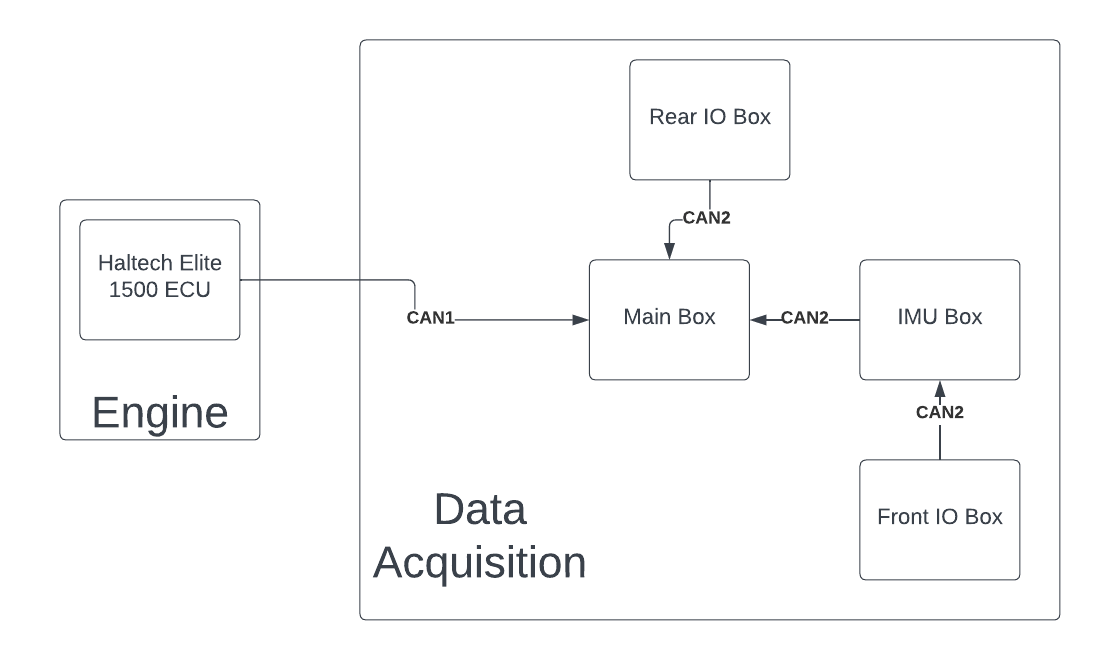
\includegraphics[width=6in]{images/SDM-23 System.png}
    \caption{SDM-23 DAQ Electrical System Block Diagram}
    \label{fig:sdm23-systemdiagram}
\end{figure}
The system block diagram in Figure \ref{fig:sdm23-systemdiagram} displays the high level components of the DAQ electrical system as well as their interfaces with each other and other electrical components in the car.
It also shows which subteam is responsible for each electrical component.
All of the DAQ components are composed of at least a custom PCB and 3D printed housing.
\vspace{1em}

The main box is the central component in SDM-23.
It is a standalone data logger that features two separate CAN bus interfaces, one used for interfacing with the Haltech ECU and the second used for interfacing with the other DAQ components, a GPS module, and a 5V regulator to step down the 12V it receives from the ECU.
\vspace{1em}

The IMU box has two functions: collecting and reading data from the ISM330DHCX, and transmitting it over CAN.
\vspace{1em}

The front and rear I/O boxes are responsible for interfacing with the majority of SDM-23's sensors and transmitting them over CAN.
For instance, the front right brake rotor temperature sensor and steering angle sensor are connected to the Front I/O box.

\section{Software Design}
The software for the SDM-23 DAQ system is relatively simple.
Figure \ref{fig:sdmioafsdasfs} shows a state diagram for the software for the IMU and IO boxes.
\begin{figure}[H]
    \centering
    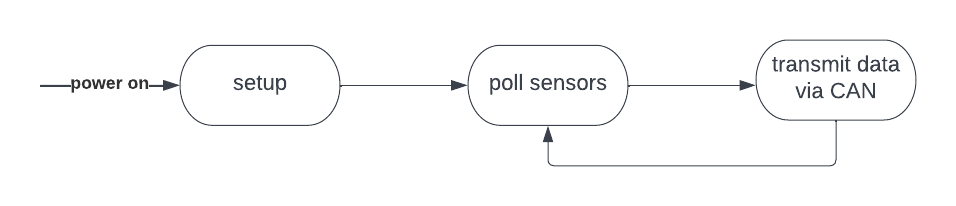
\includegraphics[width=7in]{images/sdm23software(1).png}
    \caption{State diagram for IMU and IO boxes}
    \label{fig:sdmioafsdasfs}
\end{figure}
\begin{figure}[H]
    \centering
    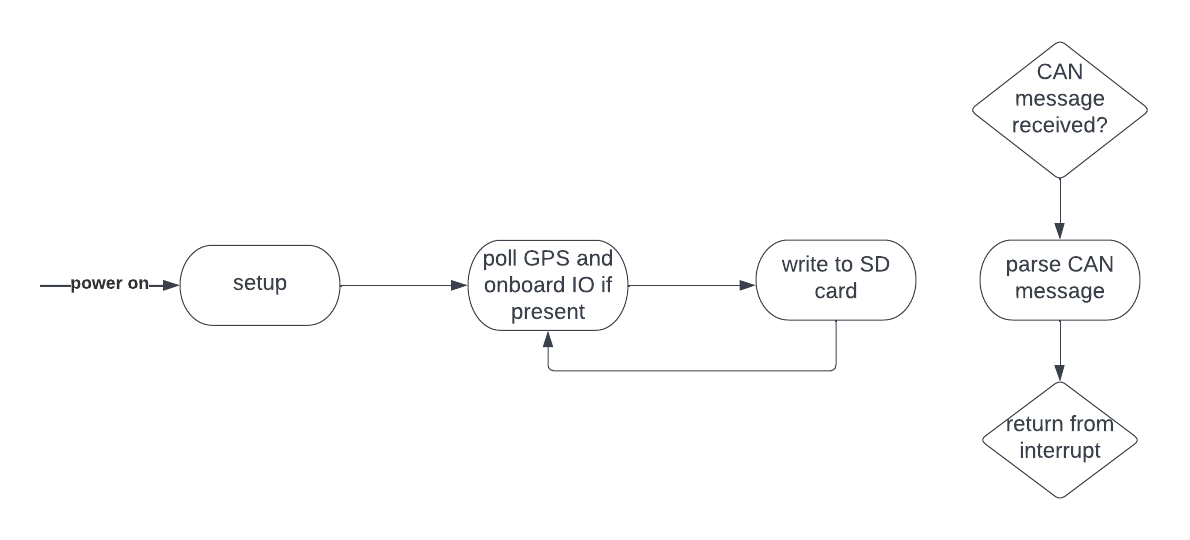
\includegraphics[width=7.5in]{images/ffff.png}
    \caption{State diagram for Main box}
    \label{fig:asdfasdfasdf}
\end{figure}
Figure \ref{fig:asdfasdfasdf} shows the state diagram for the Main box.
When the main box receives a CAN message, the SN65HVD230 triggers an interrupt for the Teensy software to parse the CAN message, returning to normal execution afterwards.
\vspace{1em}

For all boxes, once the setup function passes the onboard Teensy LED is lit up to indicate that everything has initialized successfully.

\section{Main Box Design}
The main box, using a Teensy 4.1 as its microcontroller, acts as a hub to collect data from the Haltech ECU, Front and Rear IO boxes and the IMU box via CAN.
\begin{figure}[H]
    \centering
    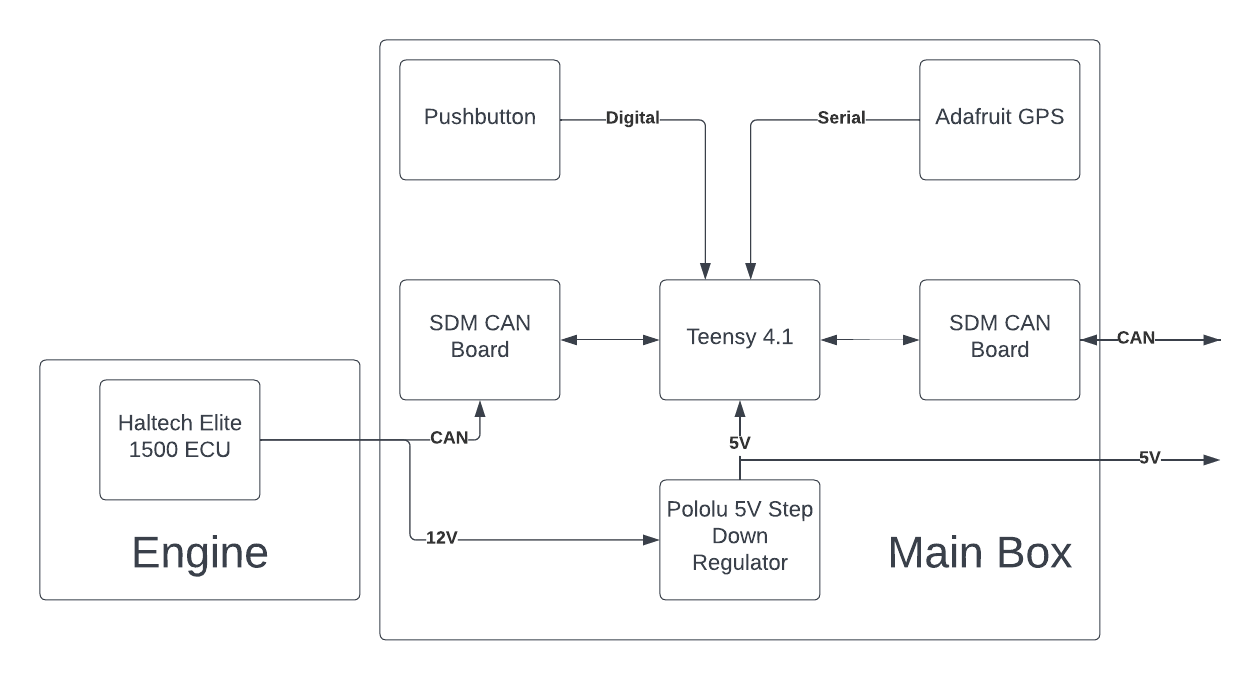
\includegraphics[width=5.5in]{images/SDM-23 Main Box Block Diagram.png}
    \caption{Main Box Block Diagram}
    \label{fig:sdm23mainboxblock}
\end{figure}

The main box includes an onboard GPS module to collect positional data and breakouts some extra I/O pins.
For data storage, the onboard Teensy 4.1's microSD card slot is used.
It receives 12V power from the ECU, which is stepped down to 5V using a Pololu 5V regulator.
The 5V is then passed to the onboard Teensy 4.1 as well as to any DAQ component connected to the main box.
It also includes a pushbutton which can be used to mark notable timestamps in order to sync with other systems (e.g., Go Pros).
\vspace{1em}

The main box also includes a panel mount micro USB connector which is connected to the Teensy 4.1's micro USB port, which will allow us to easily debug and reprogram the Teensy 4.1, and also to retrieve the data via USB.
This will greatly decrease the time and effort needed to debug the box or retrieve data, since it will no longer be necessary to disassemble the box in order to do either of the aforementioned tasks.
\vspace{1em}

The main constraint for the main box's PCB design was that it should fit within a 100mm x 100mm square, which is JLCPCB's cheapest tier for PCB manufacturing.
To cut down on assembly cost and design time, custom SN65HVD230 breakout boards were used to complete the electrical interface between the Teensy 4.1 and the CAN bus as opposed to laying out the CAN transceiver circuitry on the main board directly.
The design for the custom SN65HVD230 breakout board is detailed in Section \ref{sec:canboard}.
\vspace{1em}

The Teensy 4.1 requires $V_{in}$ to be between 3.6 and 5.5V.
However, the Haltech ECU's CAN Hub supplies 12V power.
Although the ECU is also capable of supplying 5V, upon testing of SDM-21.5 it was discovered that the DAQ electrical system requires more current than what the ECU can output on 5V.
As such, we needed a method of stepping down 12V into an acceptable level to power the Teensy 4.1.
We selected Pololu's 5V, 2.5A Step-Down Voltage Regulator to provide the Teensy 4.1 (as well as the rest of the DAQ electrical system) 5V.
By using this regulator, we were able to save time and manufacturing costs by not having to design our own voltage regulator circuitry.
\vspace{1em}

It was also decided to break out unused pins of the Teensy 4.1.
These would come in useful as we were able to connect a damper potentiometer directly to the main box during testing.
\begin{figure}[H]
    \centering
    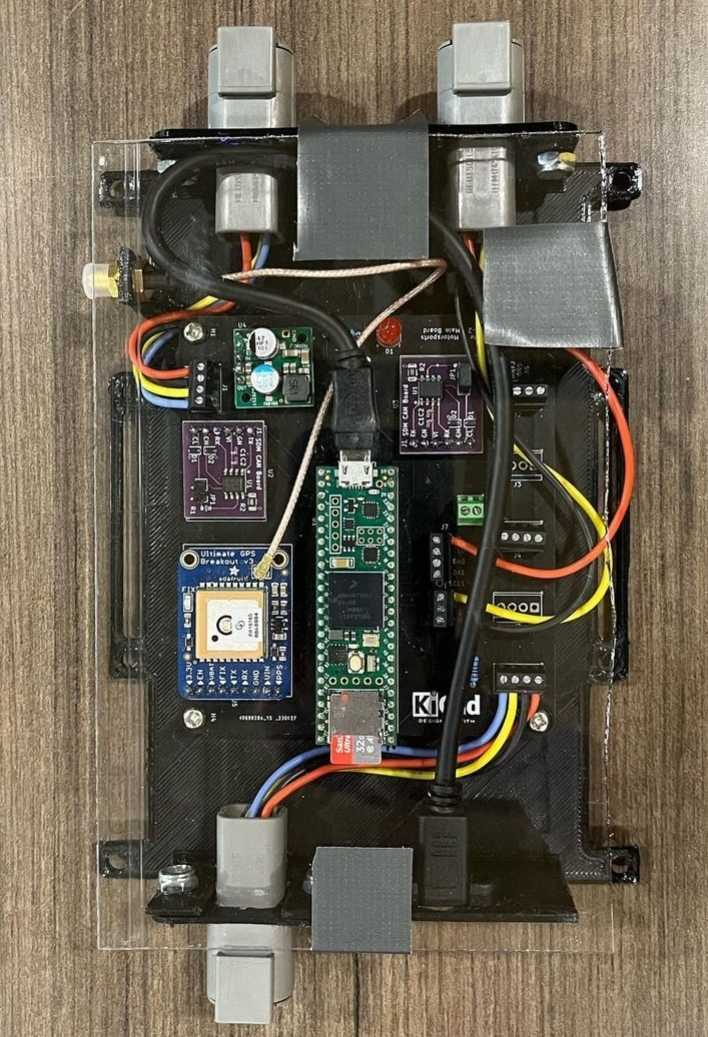
\includegraphics[width=3in,angle=90]{images/main.jpg}
    \caption{Main Box plate with assembled electronics}
    \label{fig:sdm23mainbox}
\end{figure}
\begin{figure}[H]
    \centering
    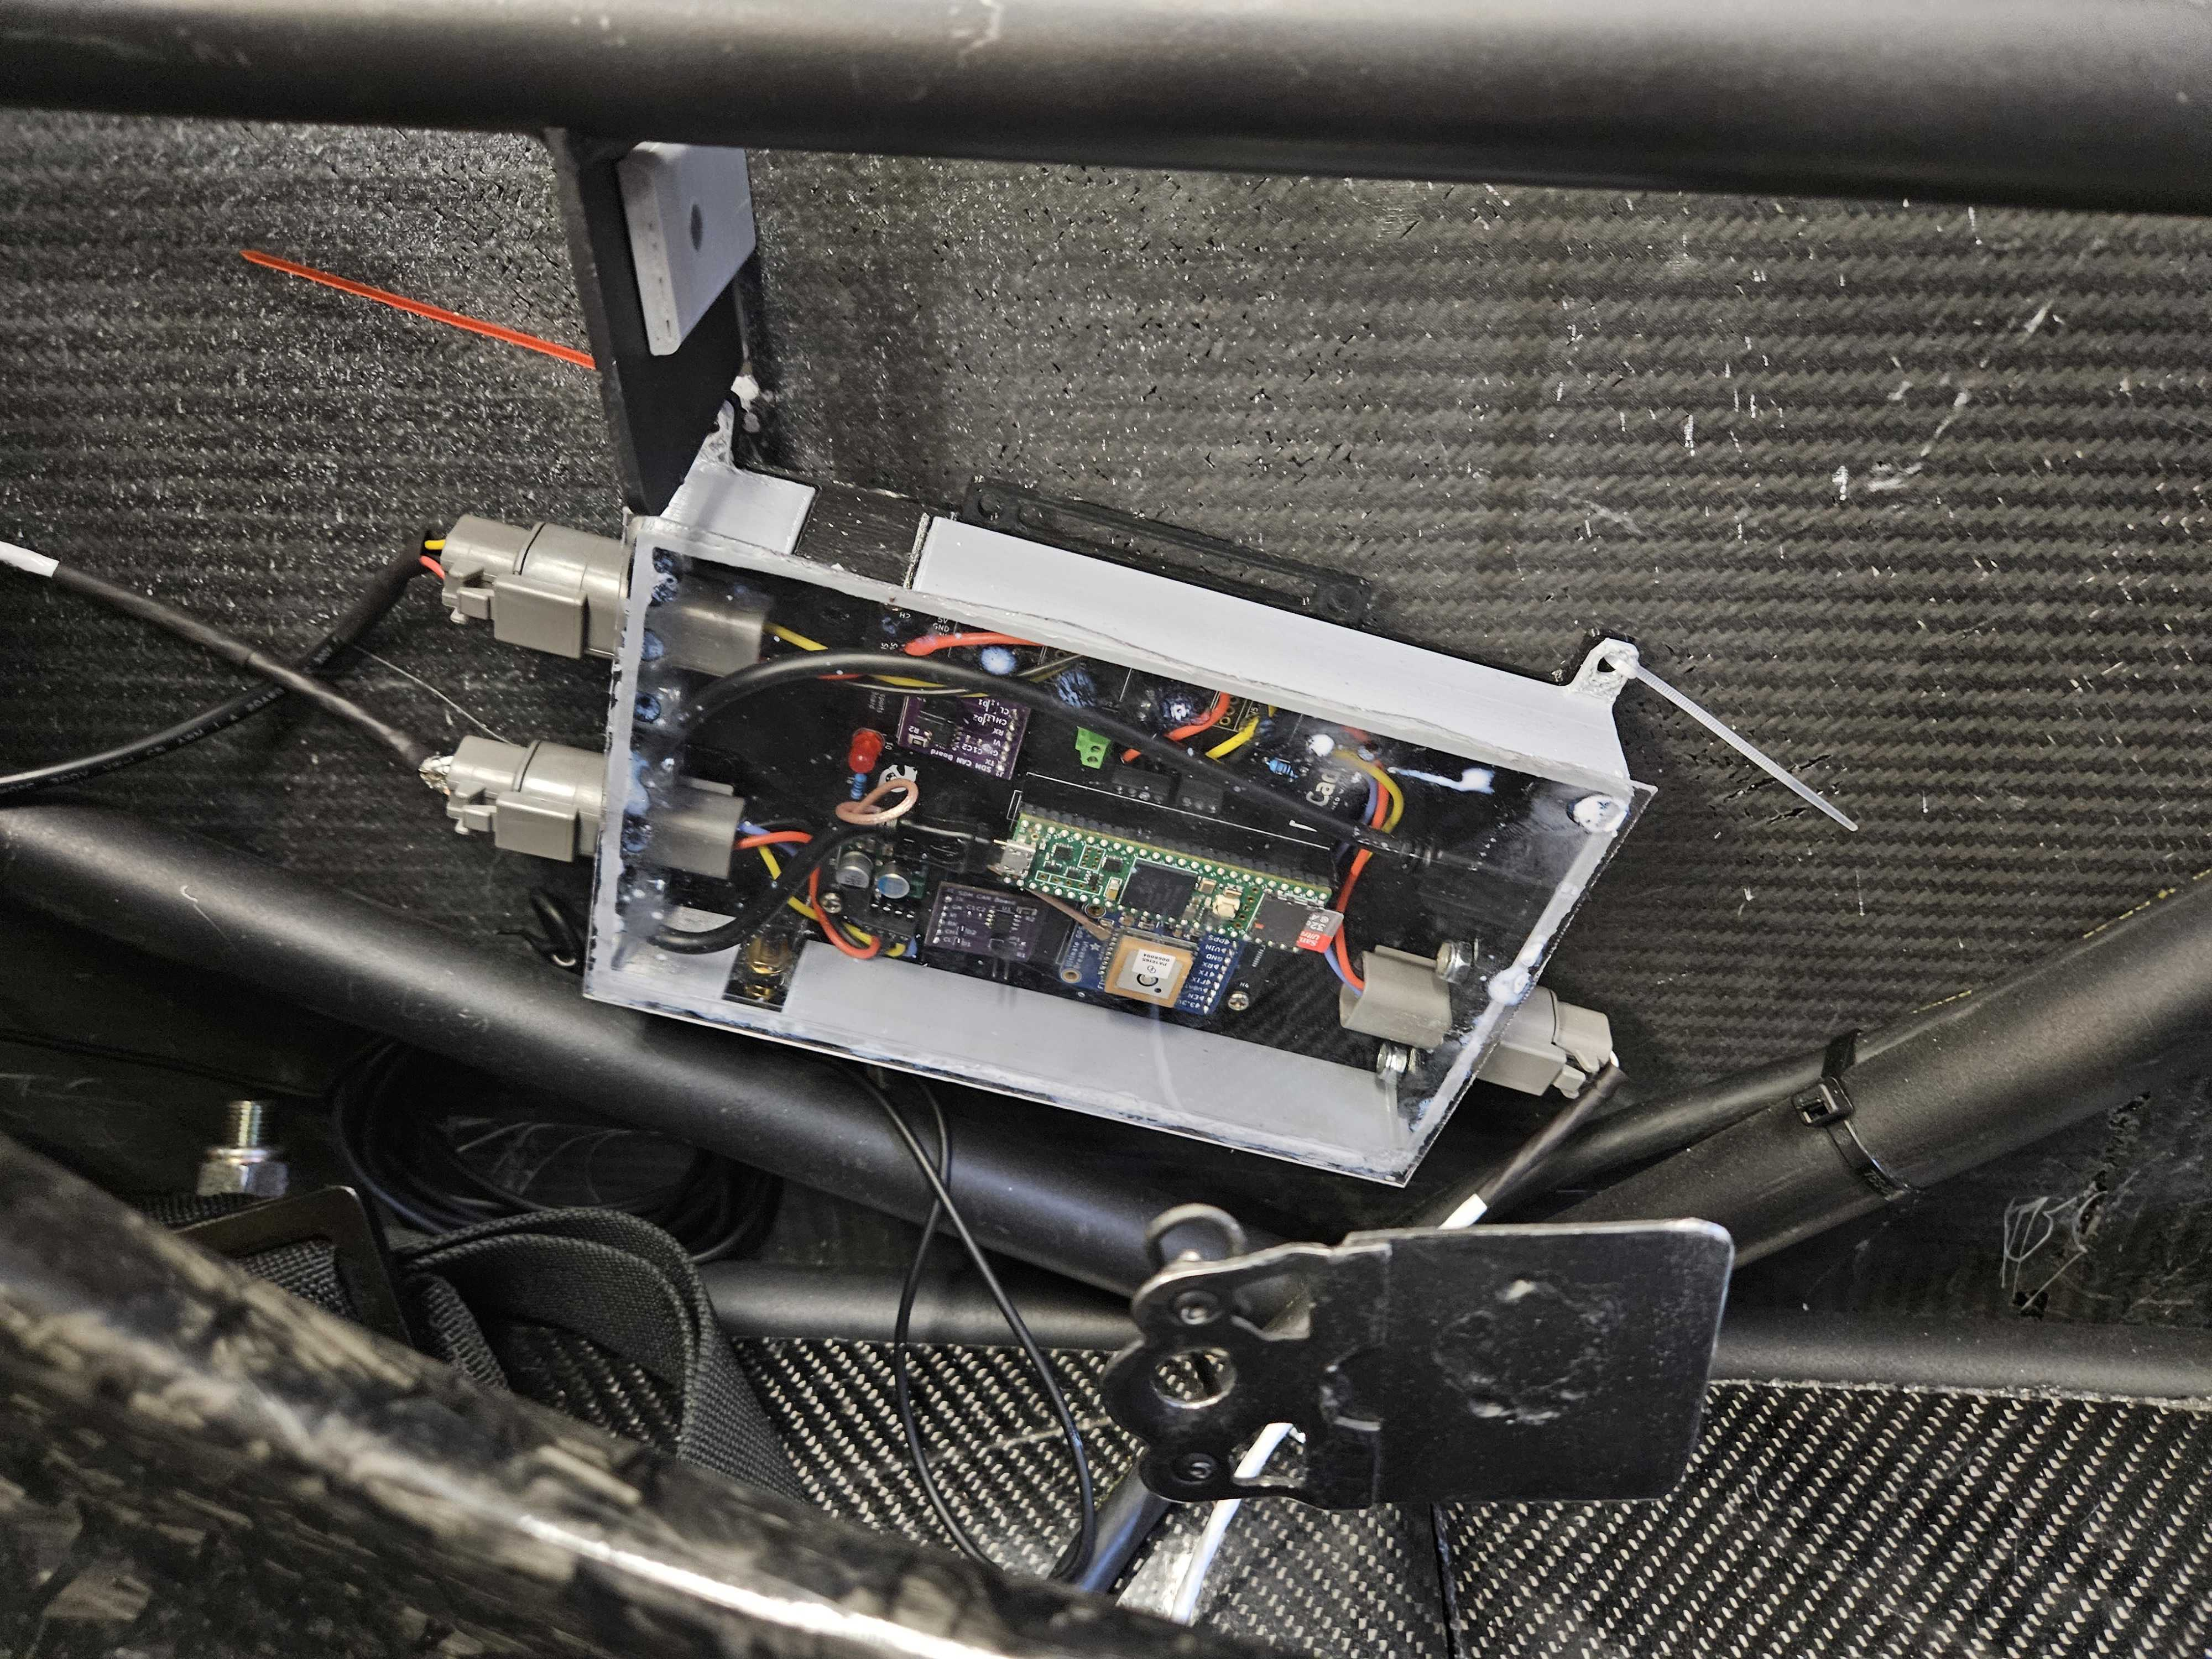
\includegraphics[width=5in]{images/asdf.jpg}
    \caption{Installed Main box in cockpit}
    \label{fig:main}
\end{figure}
The enclosure for the Main box consists of a plate that the PCB and connector panels are screwed into, a gasket, and a polycarbonate cover.
Both the plate and the gasket were 3D-printed.


\section{IMU Box Design}
The IMU box's purpose is to collect data from the ISM330DHCX and relay it to the main box via CAN.
Since the IMU box needed to be as small as possible and there was no need for onboard data storage, a Teensy 4.0 was selected to be its microcontroller.
\begin{figure}[H]
    \centering
    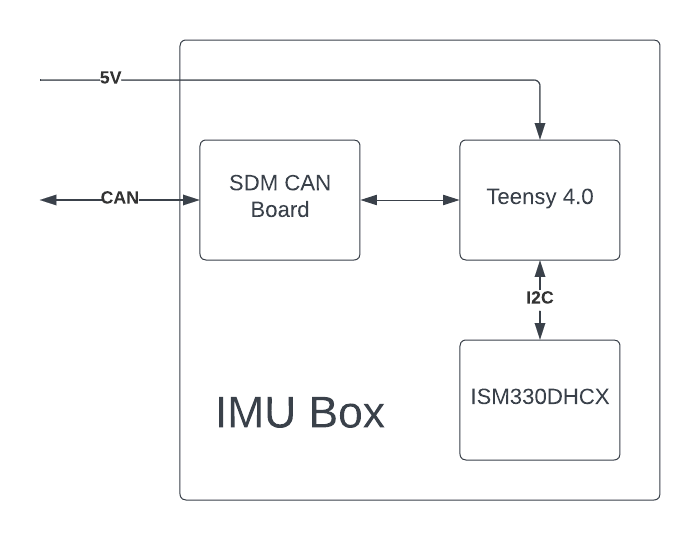
\includegraphics[width=4in]{images/SDM-23 IMU Box Block Diagram .png}
    \caption{IMU Box Block Diagram}
    \label{fig:sdm23imuboxblock}
\end{figure}
We opted to use Sparkfun's ISM330DHCX breakout board for the IMU board because we determined that it was a safer option rather than designing the IMU circuitry ourselves because we would be able to easily swap out the IMU in case it became damaged or nonfunctional for whatever reason.
\vspace{1em}

Since the IMU box was likely to be placed somewhere in the center of the car, the IMU box's pinout included a second CAN connection with 5V and GND so that we would be able to daisy chain the CAN bus, meaning that the stub length for the IMU is completely minimized.
This was able to be utilised, as the IMU box was placed underneath the driver seat and we were able to route the CAN bus from the Main box, to the IMU box, and then to the Front I/O box.
\vspace{1em}

Like the Main box, the enclosure for the IMU box consists of a 3D-printed plate and gasket and a polycarbonate cover.
\begin{figure}[H]
    \centering
    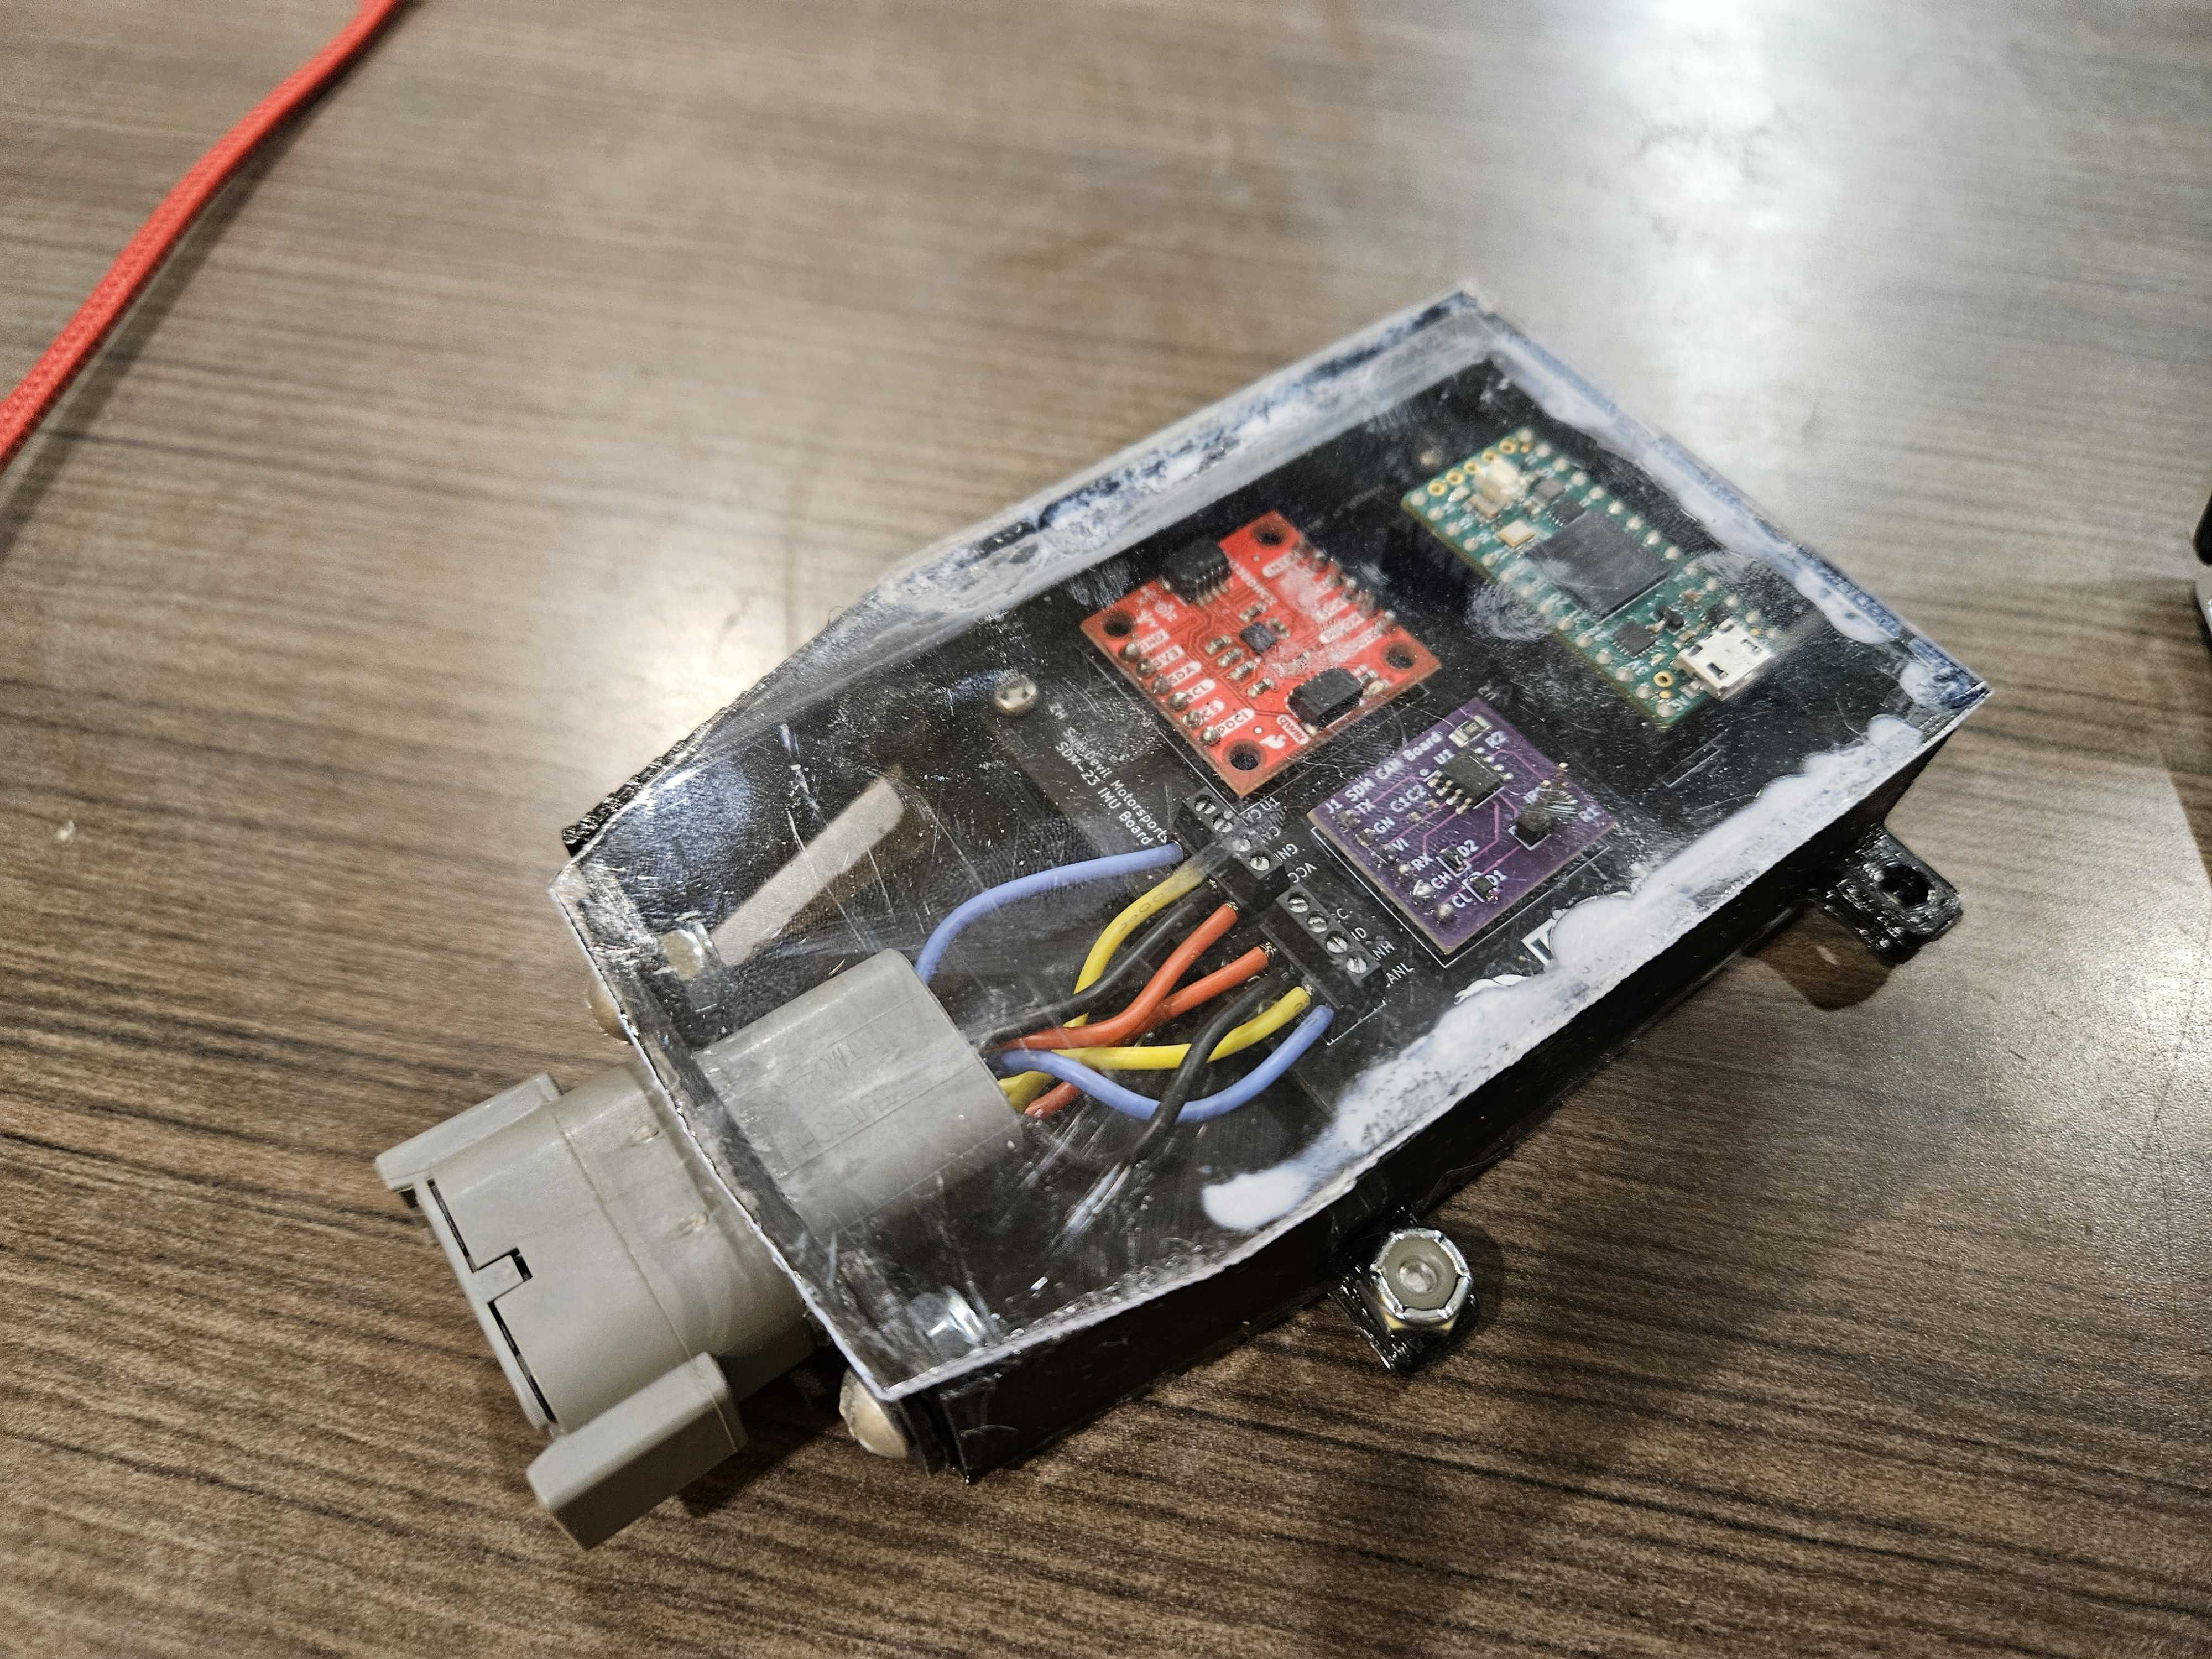
\includegraphics[width=4in]{images/imuimu.jpg}
    \caption{Assembled IMU box}
    \label{fig:sdm23imubox}
\end{figure}
\subsection{Gyroscope Debugger}
To assist in tuning the gyroscope to produce as clean data as possible, a debugging software was developed to plot and integrate the angular rate produced by the gyroscope.
It works by the Teensy 4.0 relaying gyroscope data to a computer via USB Serial.
The debugger then parses the data and plots it using \texttt{pyqtgraph}.
The software also gives the option for the user to input a zero value to use for integration, and includes a model of SDM-23 to visualize the car's angular position.
\begin{figure}[H]
    \centering
    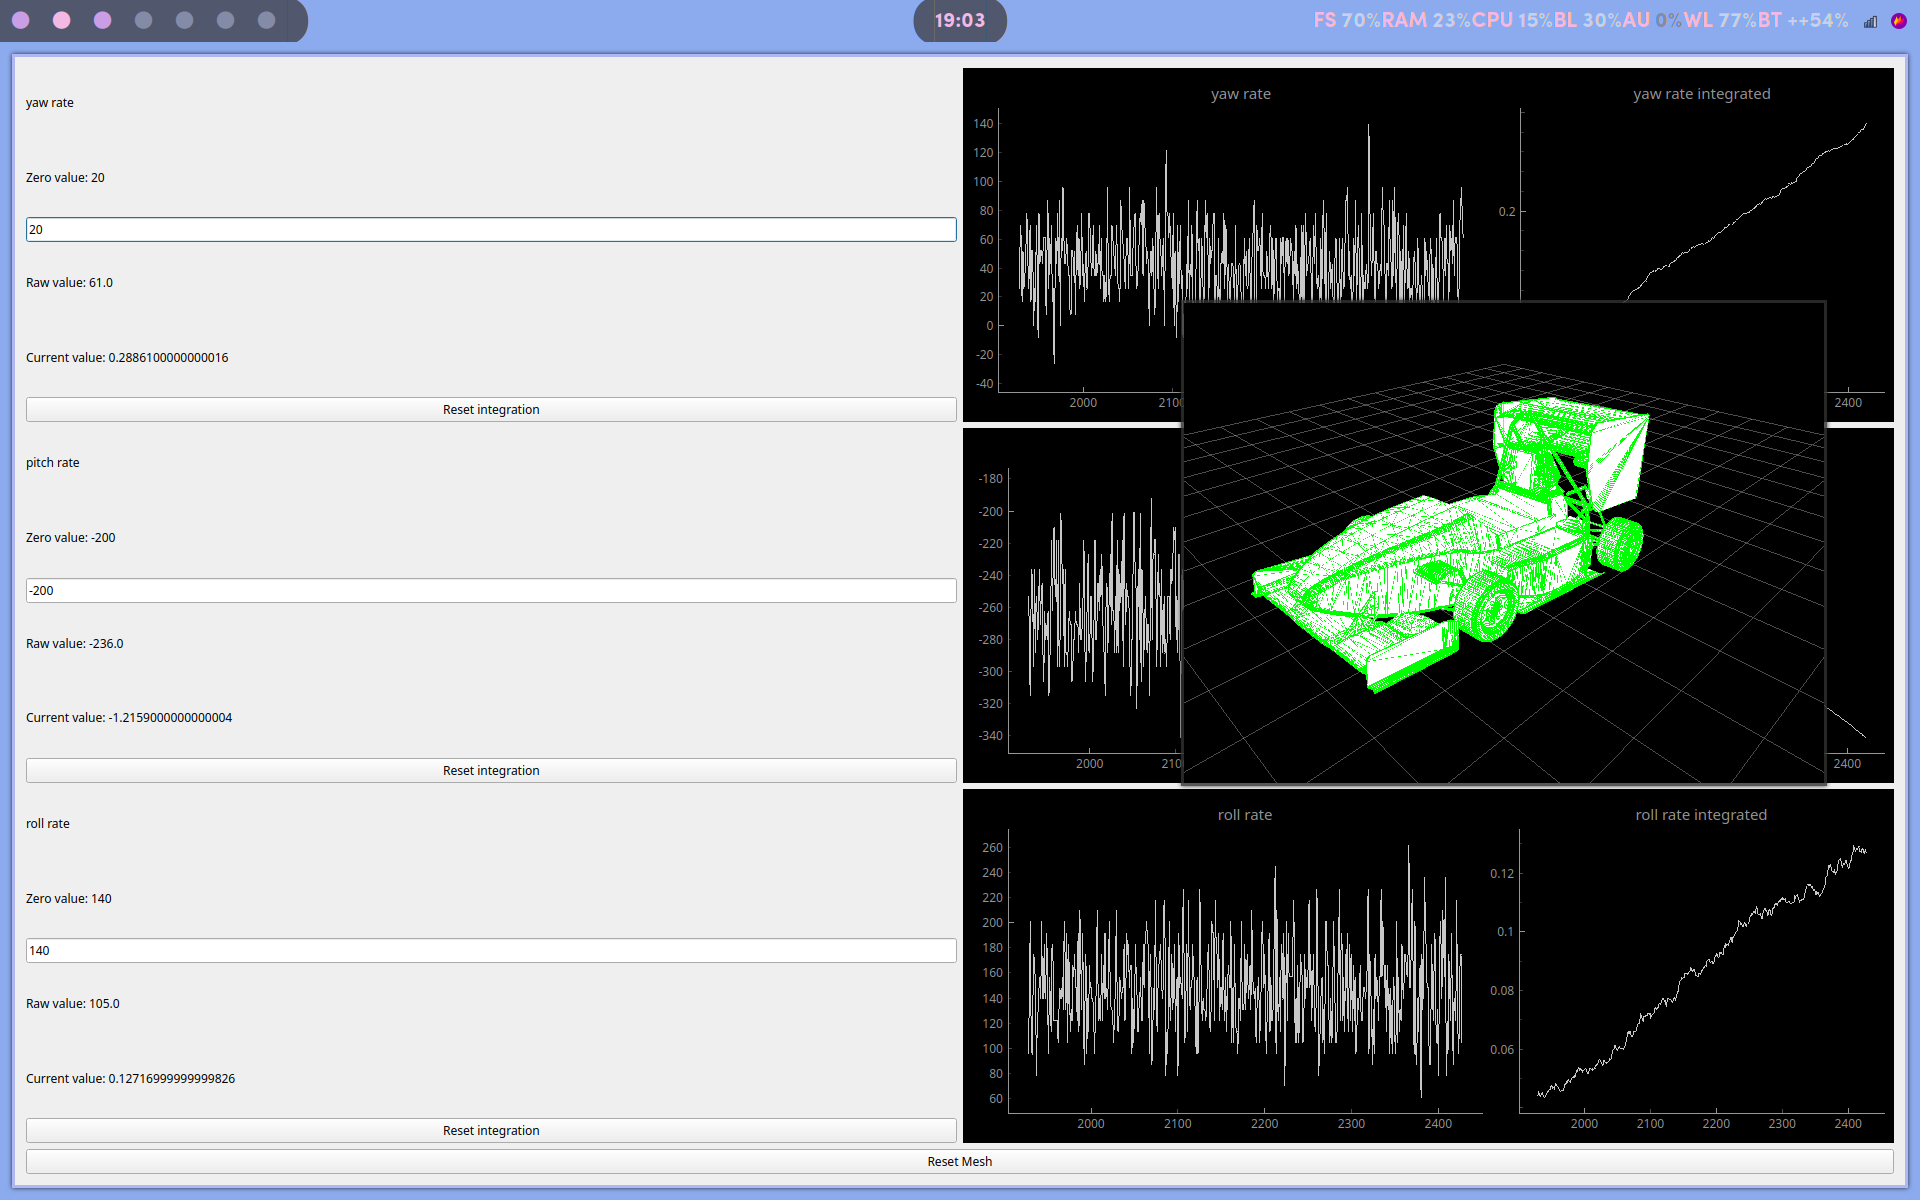
\includegraphics[width=7in]{images/debug.png}
    \caption{Gyroscope debugger software}
    \label{fig:deb}
\end{figure}

\section{Front/Rear IO Box Design}
The I/O Boxes are responsible for interfacing with the majority of SDM-23's sensors.
Its primary components are a Teensy 4.0 and a CAN transceiver board.
\begin{figure}
    \centering
    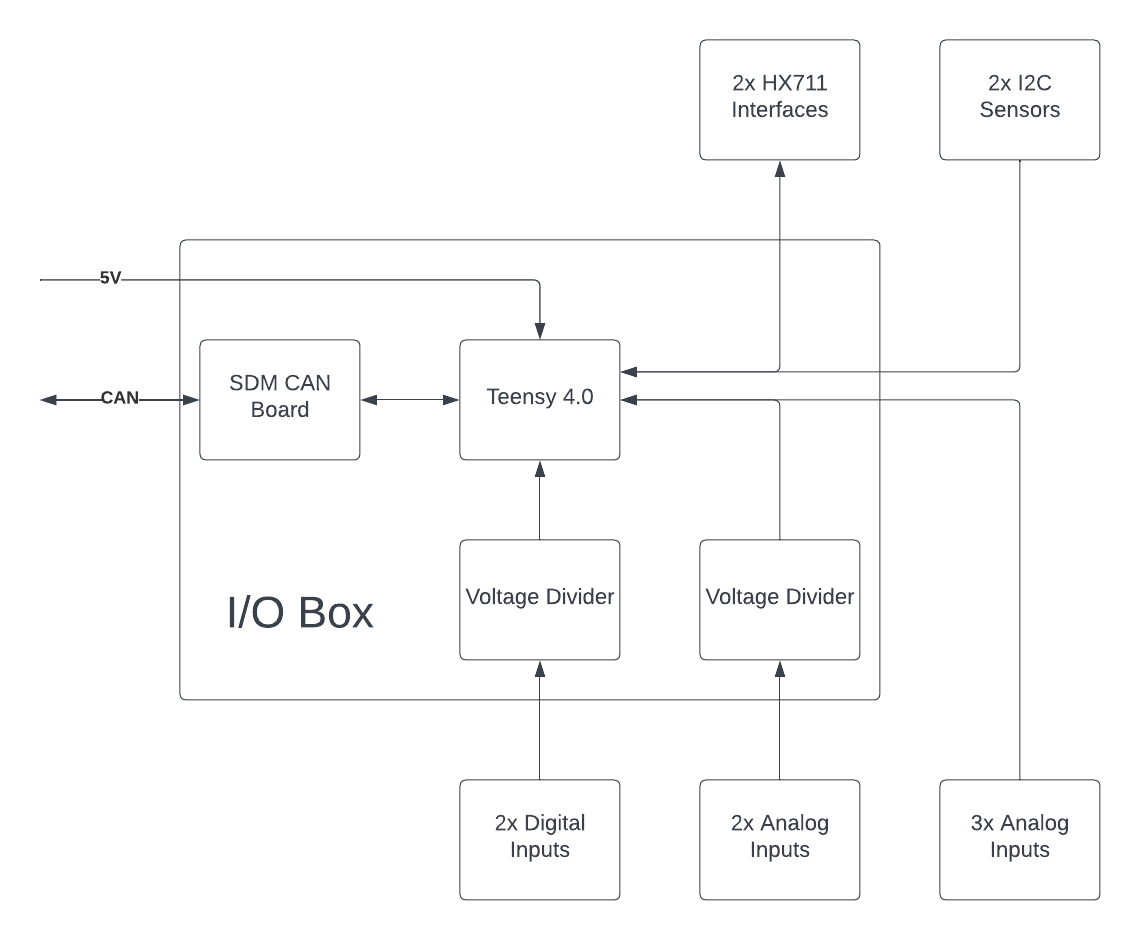
\includegraphics[width=5in]{images/SDM-23 IO Box Block Diagram.png}
    \caption{I/O Box Block Diagram}
    \label{fig:sdm23ioboxblock}
\end{figure}
It includes pinouts for:
\begin{itemize}
    \item 2x 5V digital inputs
    \item 2x 5V analog inputs
    \item 3x 3.3V analog inputs
    \item 2x 3.3V I2C sensors
    \item 2x HX711 interfaces
\end{itemize}
It was designed to be agnostic enough where it can be used in any car produced by the team.
For SDM-23, the Front I/O makes use of both HX711 interfaces, both 5V analog inputs for the brake pressure sensors, one I2C sensor for the brake temperature sensor, and one 3.3V analog input for the steering angle sensor.
\vspace{1em}

The box has one DTM-4 connector for the CAN connection, and 3 DTM-12 connectors, where one connector would be for sensors on the front left side of the car, one would be for sensors on the front right side, and one would be for other sensors.

\begin{figure}
    \centering
    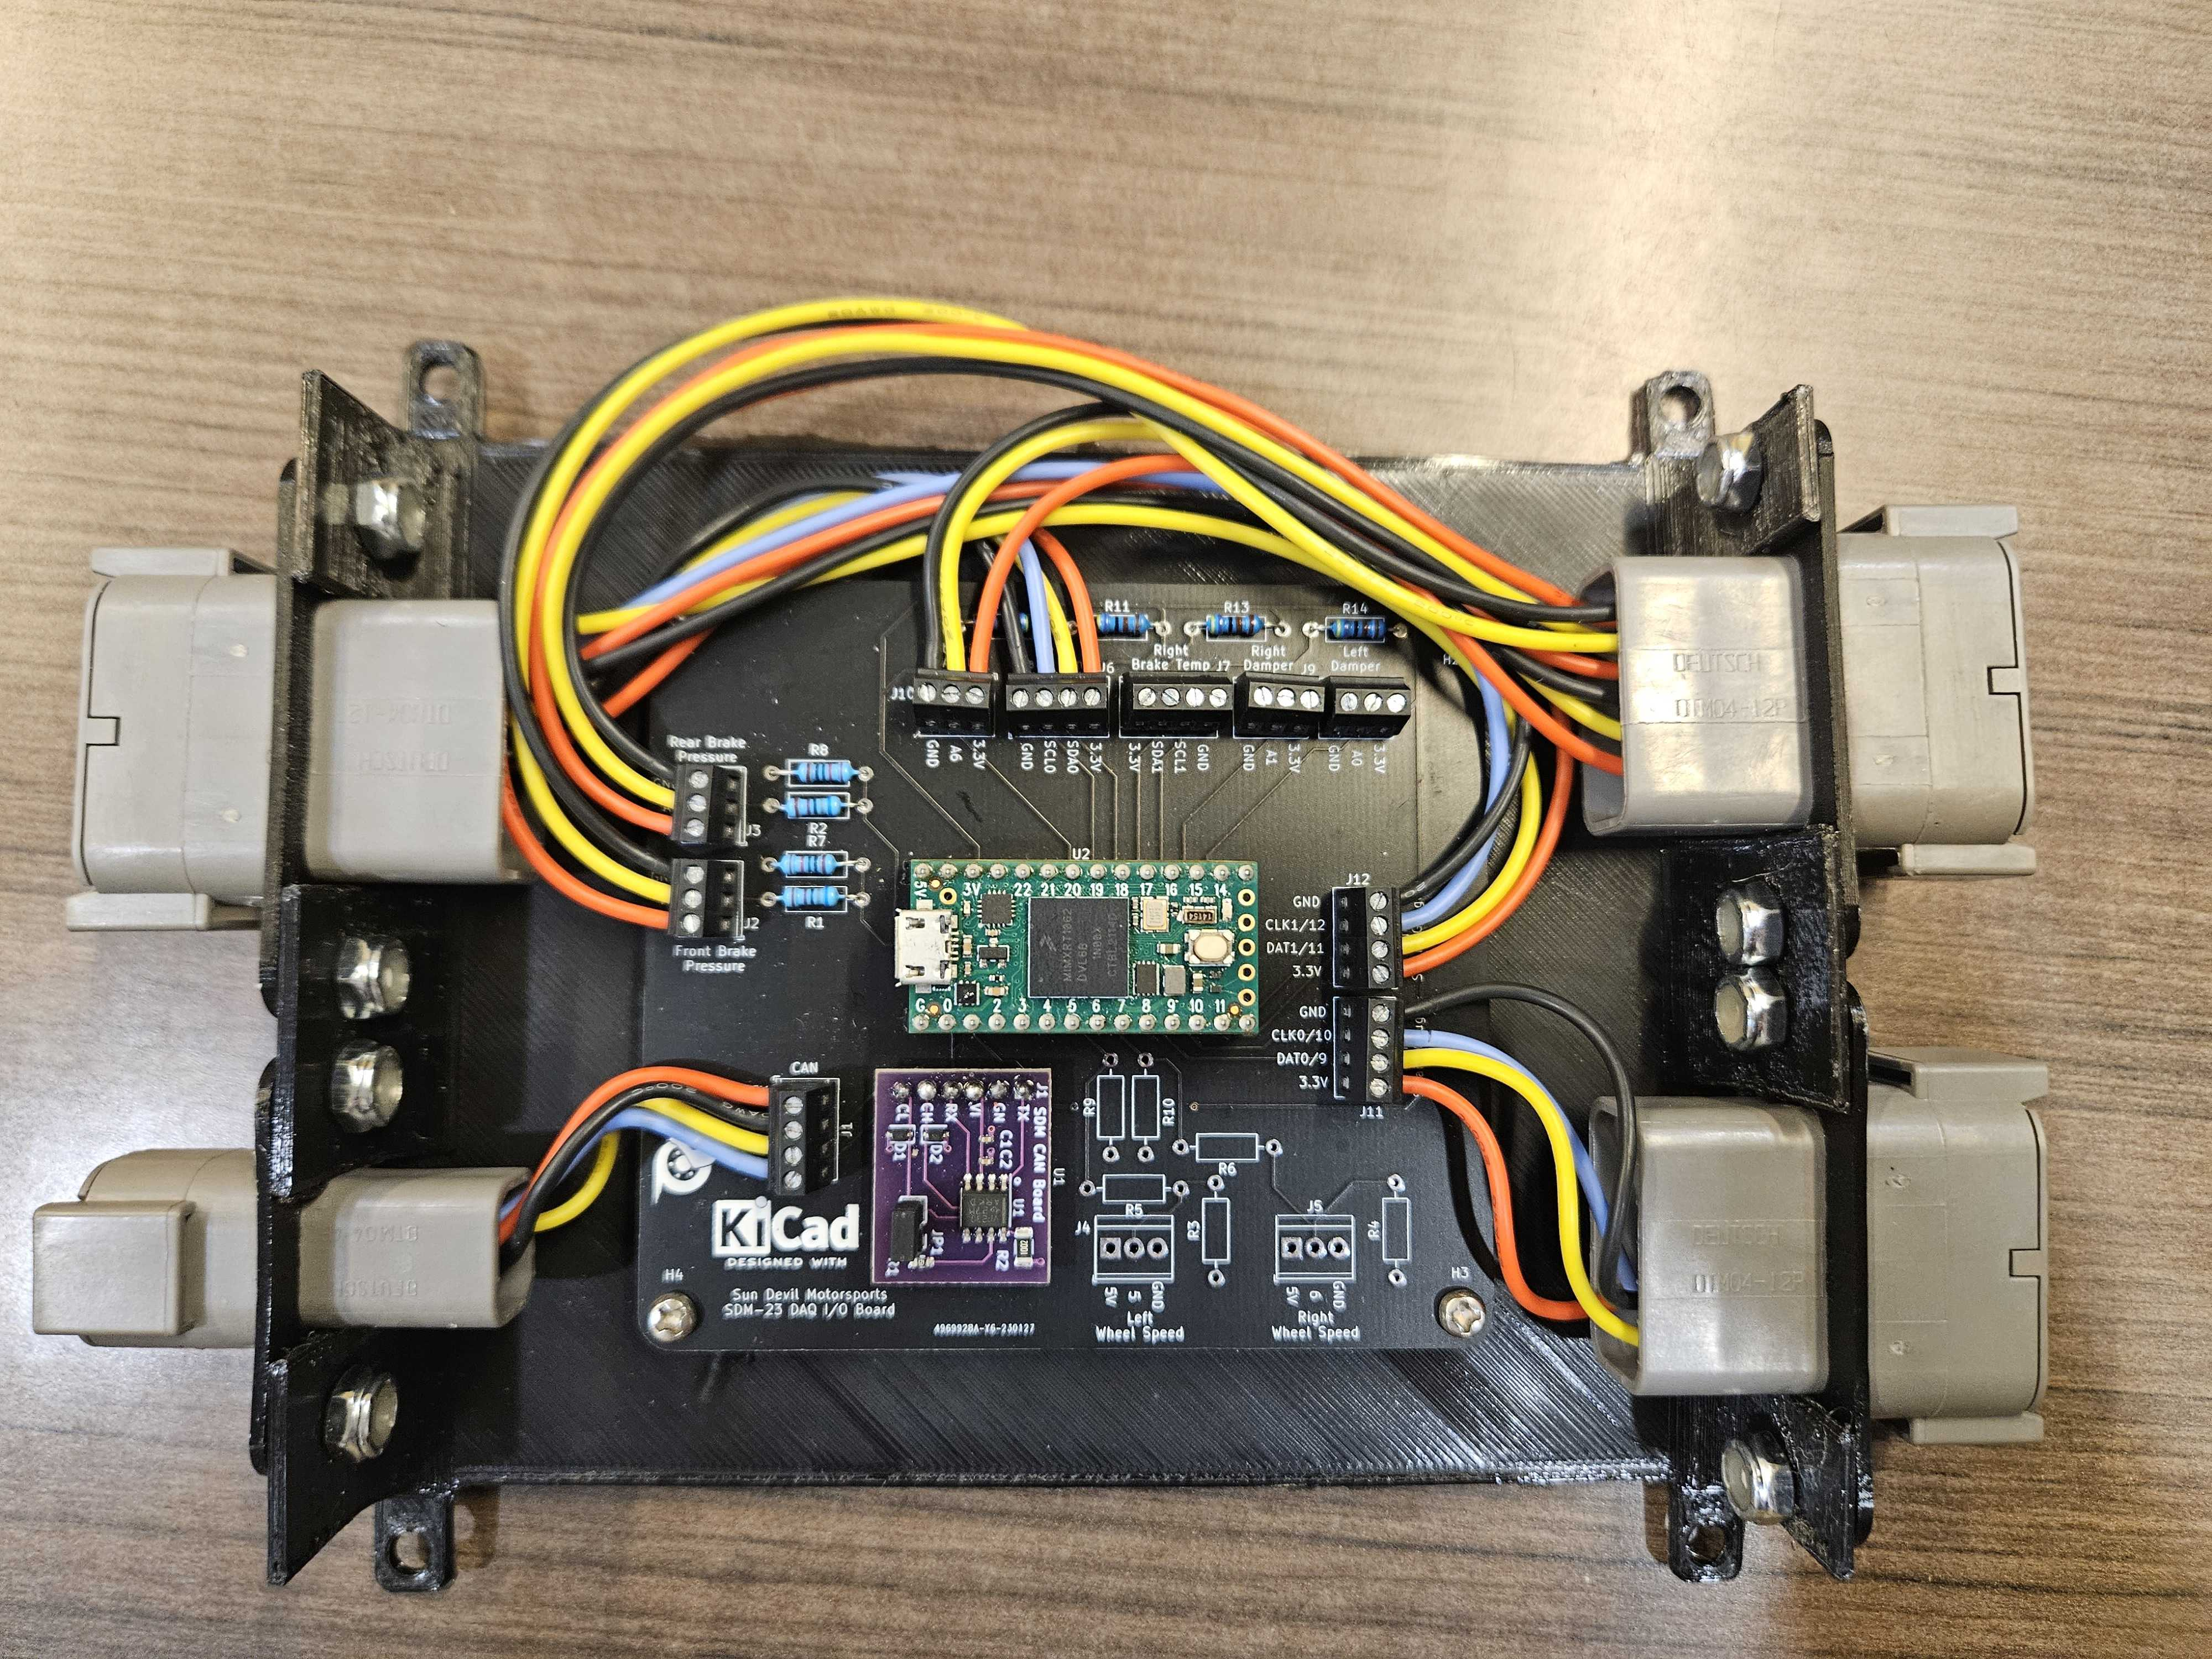
\includegraphics[width=5in]{images/io.jpg}
    \caption{IO Box plate with assembled electronics for front I/O}
    \label{fig:io}
\end{figure}

2.7k$\Omega$ Pull-up resistors for the I2C sensors are built-in to the PCB, and the voltage dividers use 6.8k$\Omega$ and 10k$\Omega$ resistors for $R_1$ and $R_2$ respectively to step down 5V into a 3V range.



\section{CAN Transceiver Board Design}\label{sec:canboard}
The CAN transceiver board provides a pinout for the SN65HVD230 CAN transceiver.
Since virtually all of the boards designed for this package requires a CAN transceiver and its supporting circuitry, a breakout board was designed so that we would design the circuitry once and be able to implement it on all of the boards in the package.
This would also allow us to test and prototype circuitry for the DAQ package on breadboards before the PCB designs were manufactured.
\vspace{1em}

A custom breakout board was designed as opposed to purchasing a commercial off-the-shelf solution because many boards available for purchase had a $120\Omega$ resistor soldered directly, meaning that if a node wasn't supposed to be terminating the resistor had to be completely desoldered.
So a design goal for this board was to include optional termination, where a jumper could be added if the resistor needed to be used.
\vspace{1em}

The SN65HVD230 comes with integrated slope control, which adjusts the output rise and fall slopes.
If the $R_S$ pin is strongly pulled to ground it is in high speed mode, where the output is allowed to switch as fast as possible.
If a $10k\Omega$ to $100k\Omega$ resistor is connected between $R_S$ and ground, then it is in slope control, where the output's slope is controlled and does not switch as fast.
This reduces the electromagnetic interference produced by the rise and fall times of the driver and resulting harmonics.
For this reason it was chosen to put the SN65HVD230 in slope control by connecting a $10k\Omega$ resistor between $R_S$ and ground.
\vspace{1em}

The rest of the supporting circuitry on the board such as bypass capacitors and ESD protection was guided by Texas Instruments' layout guidelines found in the SN65HVD230's datasheet.

\begin{figure}[H]
    \centering
    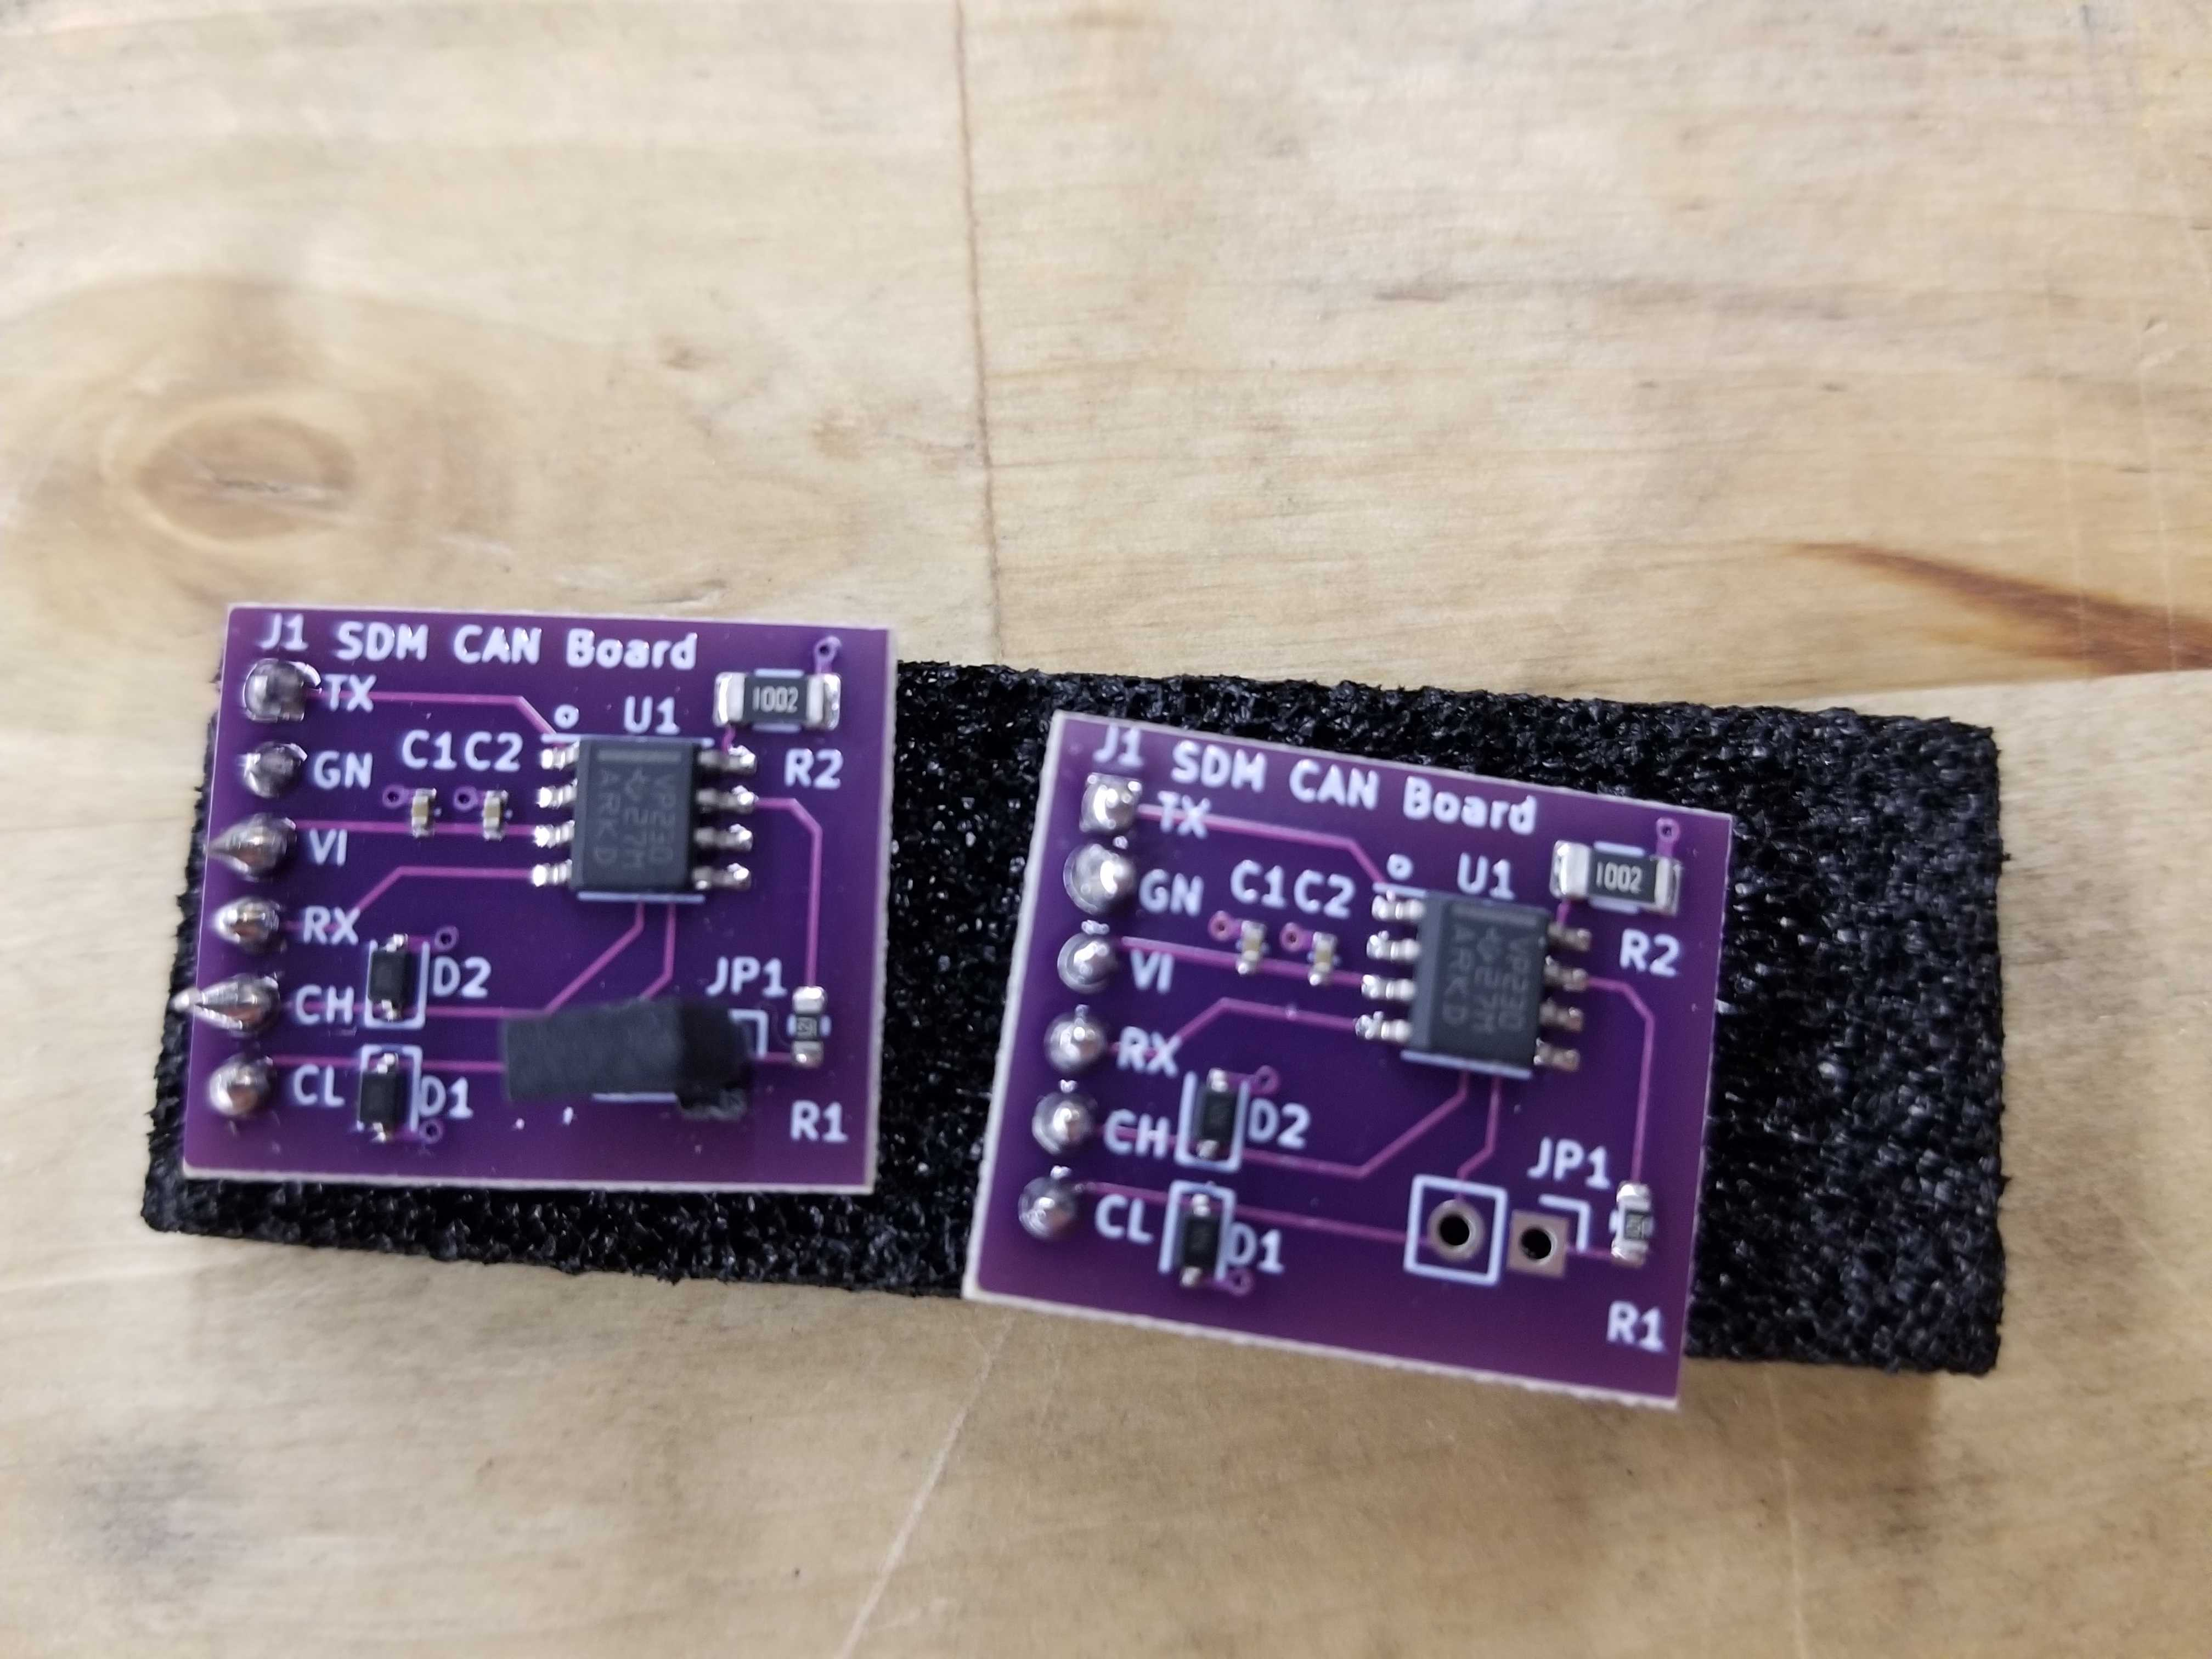
\includegraphics[width=4in]{images/sdmcanboardv1.jpg}
    \caption{CAN Transceiver Board}
    \label{fig:sdmcanboard}
\end{figure}


\section{Damper Potentiometer Design}
Linear potentiometers are used to measure the dampers' displacement and speed.
The design for the damper potentiometer consists of aluminum brackets, 3D-printed body and slide, and the linear potentiometer itself.
The 3D-printed portions of the design are mostly carried over from SDM-22, with the exception of the mounting holes and the filament used.
Instead of mounting the 3D-printed parts directly to the damper, these parts would be attached to aluminum brackets, which would attach to the damper.
In doing so, large spacers would not required to mount the potentiometer.
\begin{figure}[H]
    \centering
    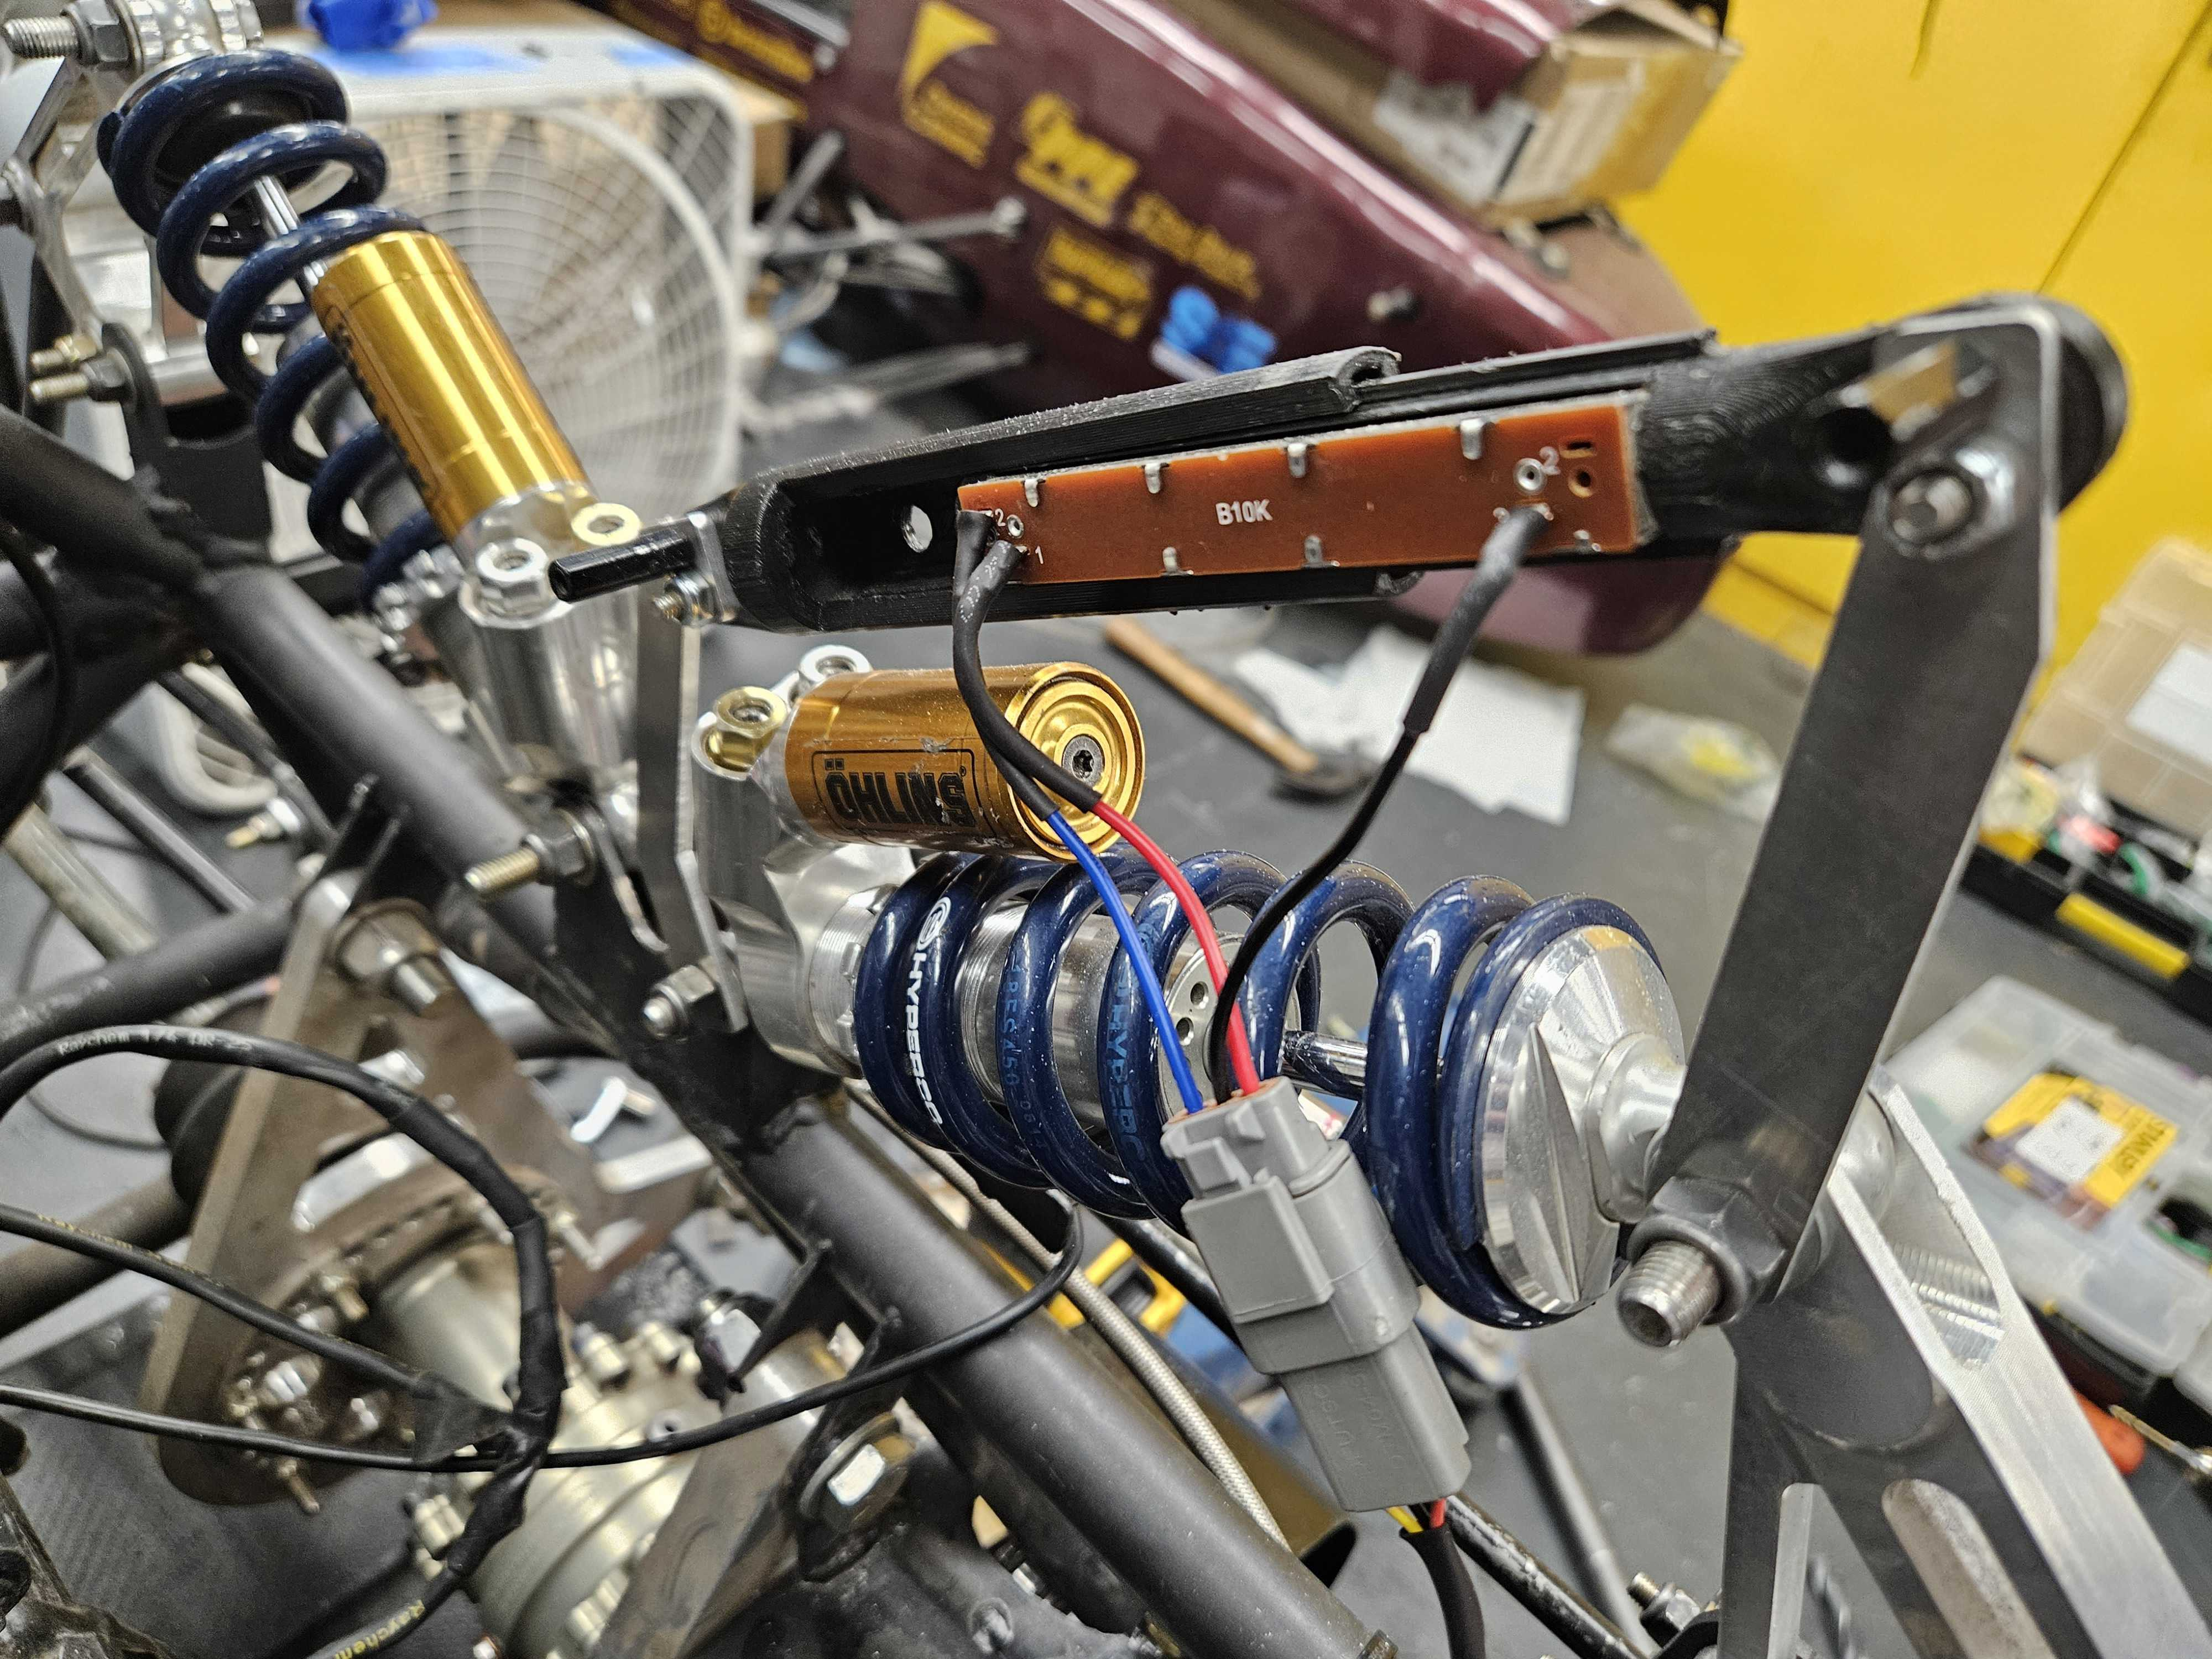
\includegraphics[width=3in]{images/pots.jpg}
    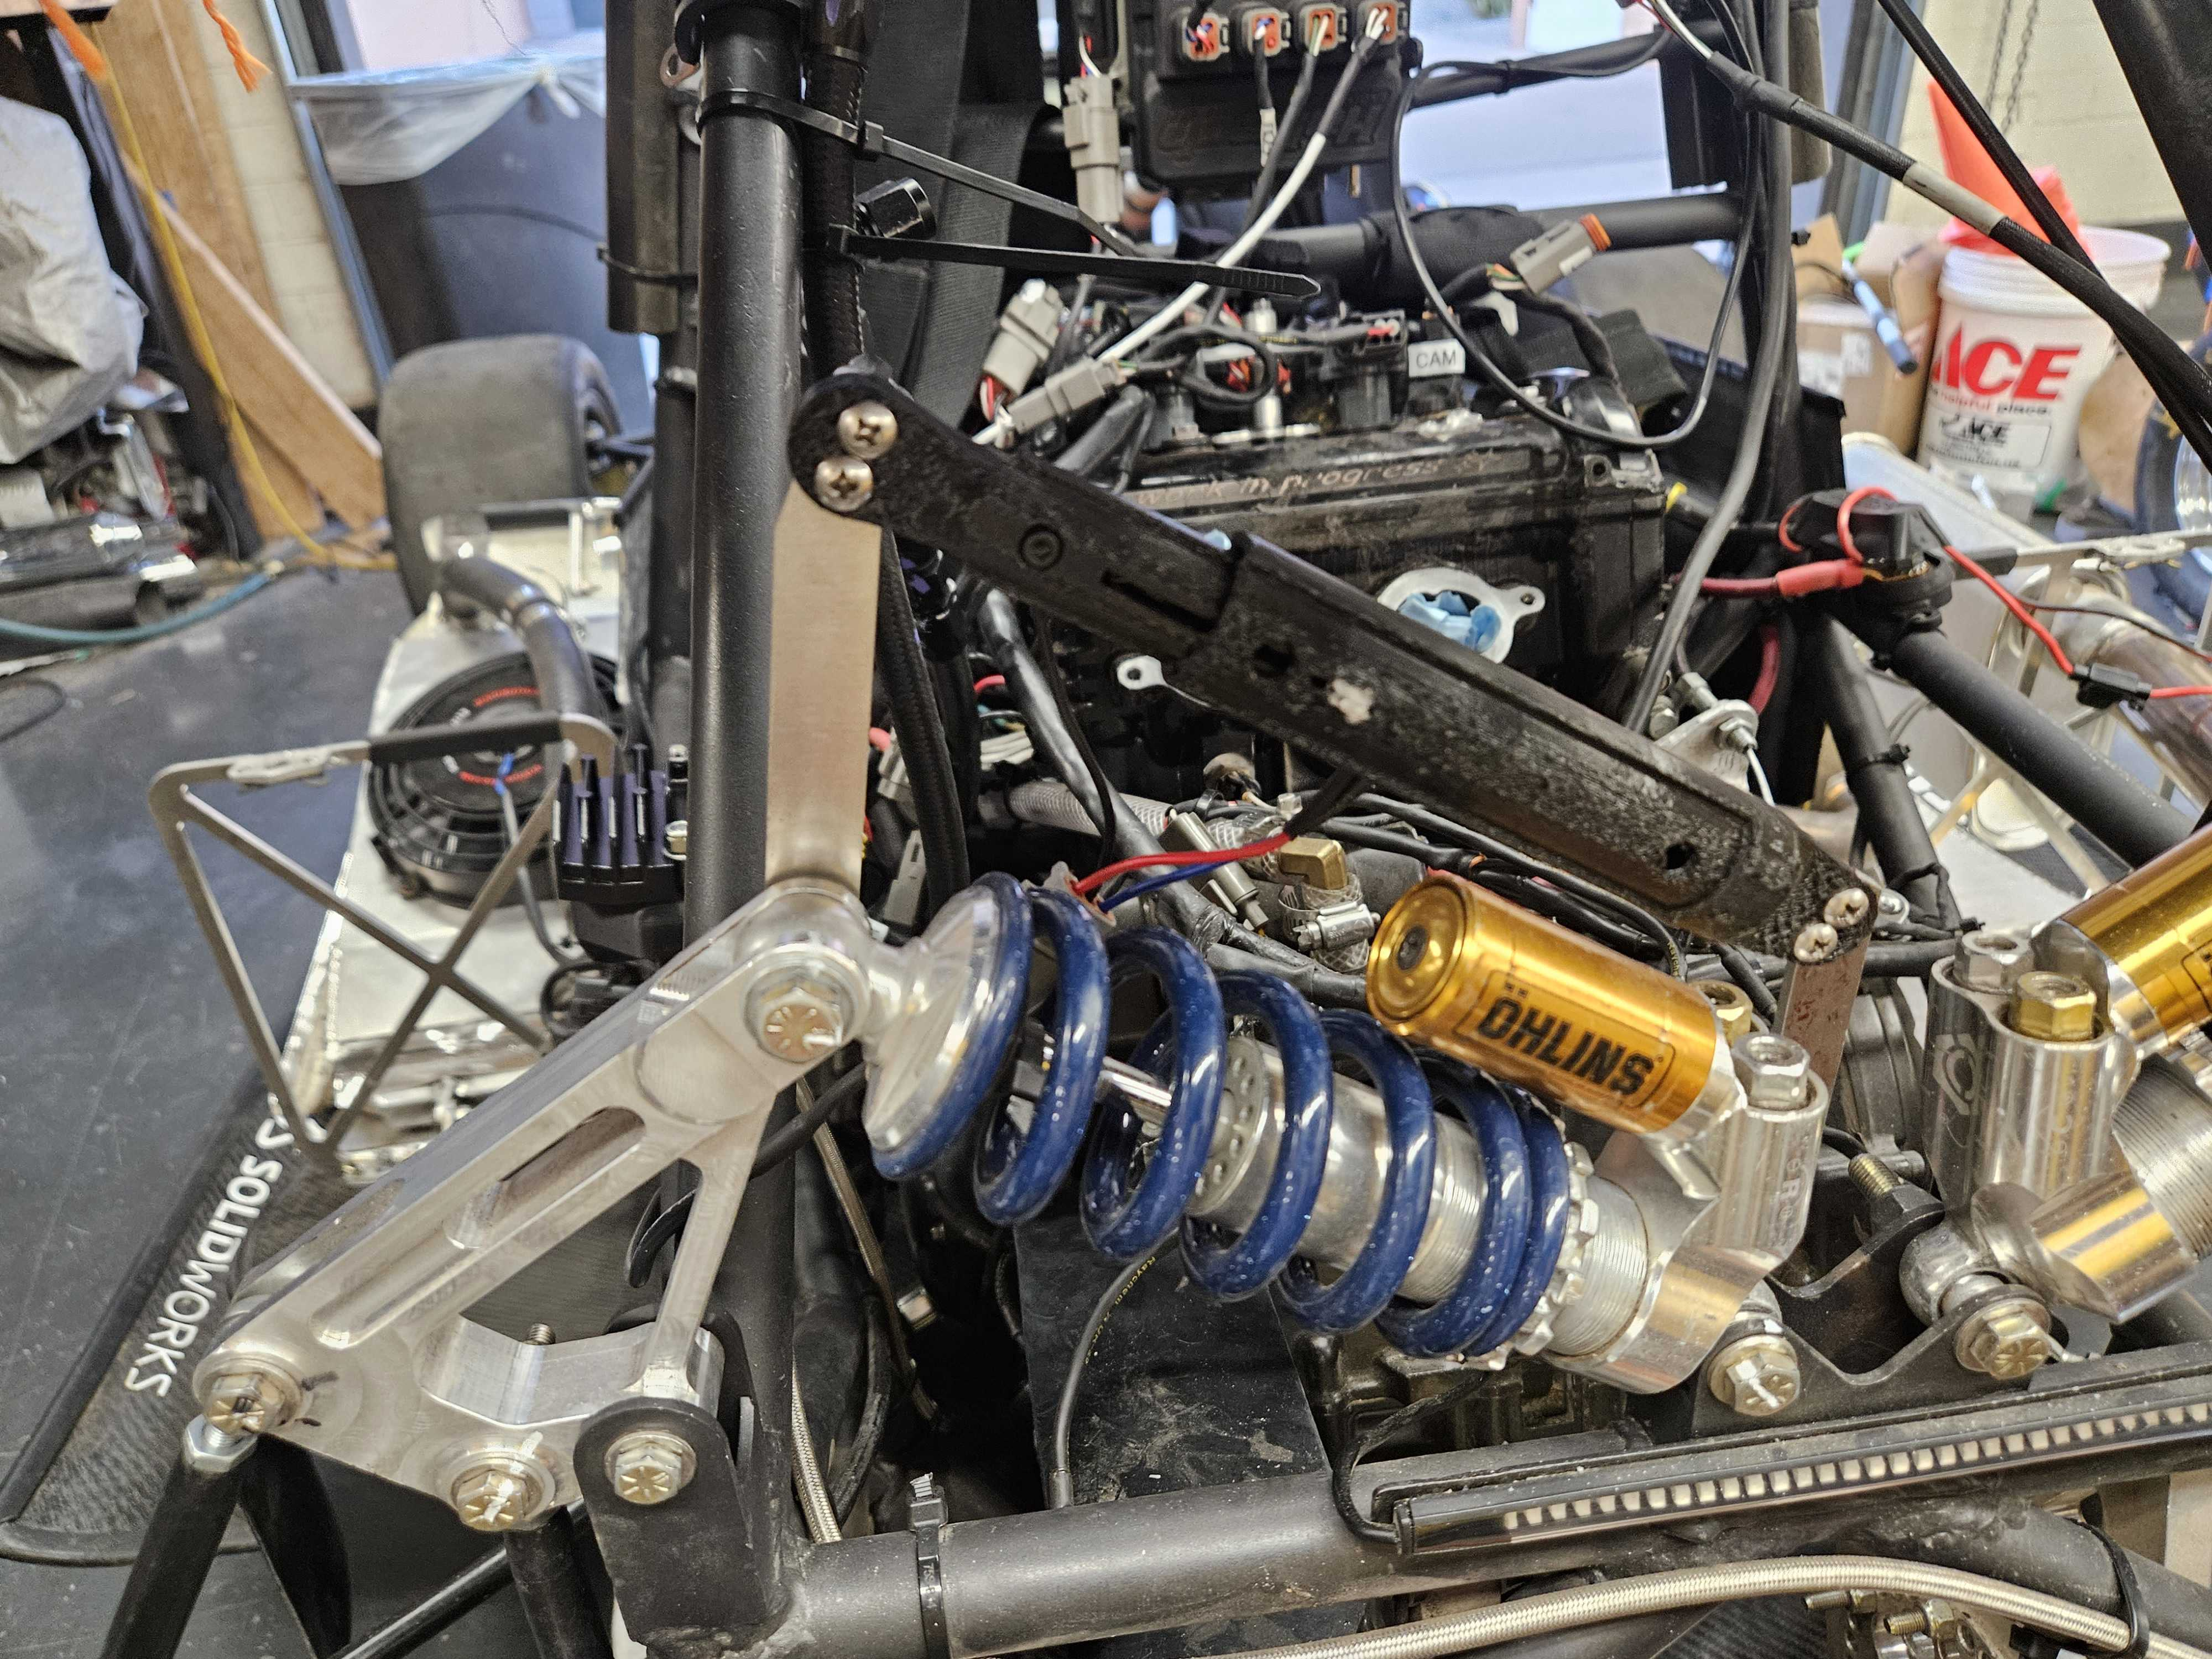
\includegraphics[width=3in]{images/potu.jpg}
    \caption{Damper Potentiometer}
    \label{fig:dp}
\end{figure}
\vspace{1em}

PETG was used instead of ASA to print the 3D-printed parts because PETG is able to bend more before shattering, as this was an issue in prior years.

\section{Steering Angle Sensor Design}
The steering angle sensor consists of the rotary potentiometer, an adapter for the potentiometer knob, and a mount to secure the potentiometer to the steering rack.
The Kaz Technologies Steering Rack includes a keyhole at the bottom of the steering rack around where the steering column is, so the adapter for the potentiometer was designed to fit into this keyhole.
The mount also screws in to 8-32 holes located at the bottom of the steering rack.
\begin{figure}[H]
    \centering
    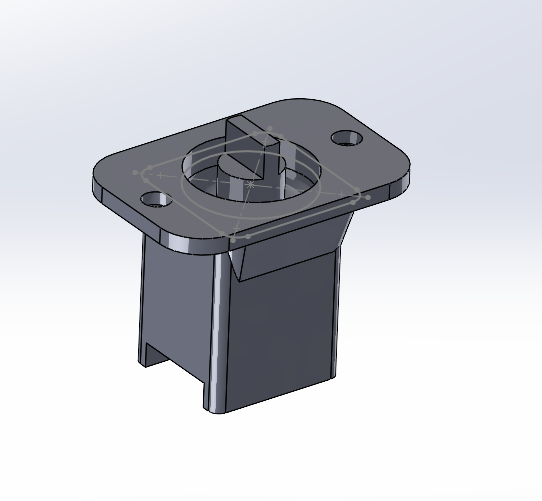
\includegraphics[width=3in]{images/steering.png}
    \caption{Steering Angle Sensor CAD}
    \label{fig:sasc}
\end{figure}

An alternative method of mounting the potentiometer to measure steering angle was a belt and pulley system.
However, given that this method is more complex, we opted to mount the potentiometer at the bottom of the steering rack.

\section{Brake Temperature Sensor Design}
The brake temperature sensor consists of the MLX90614 and a 3D-printed upright mount.
The MLX90614 IR Thermometer is used to measure the temperature of the brake rotors.
The upright mount was printed in PETG, and is designed to clip onto the upright and be secured with an existing fastener.
The MLX90614 is then secured to the mount via super glue.
\begin{figure}[H]
    \centering
    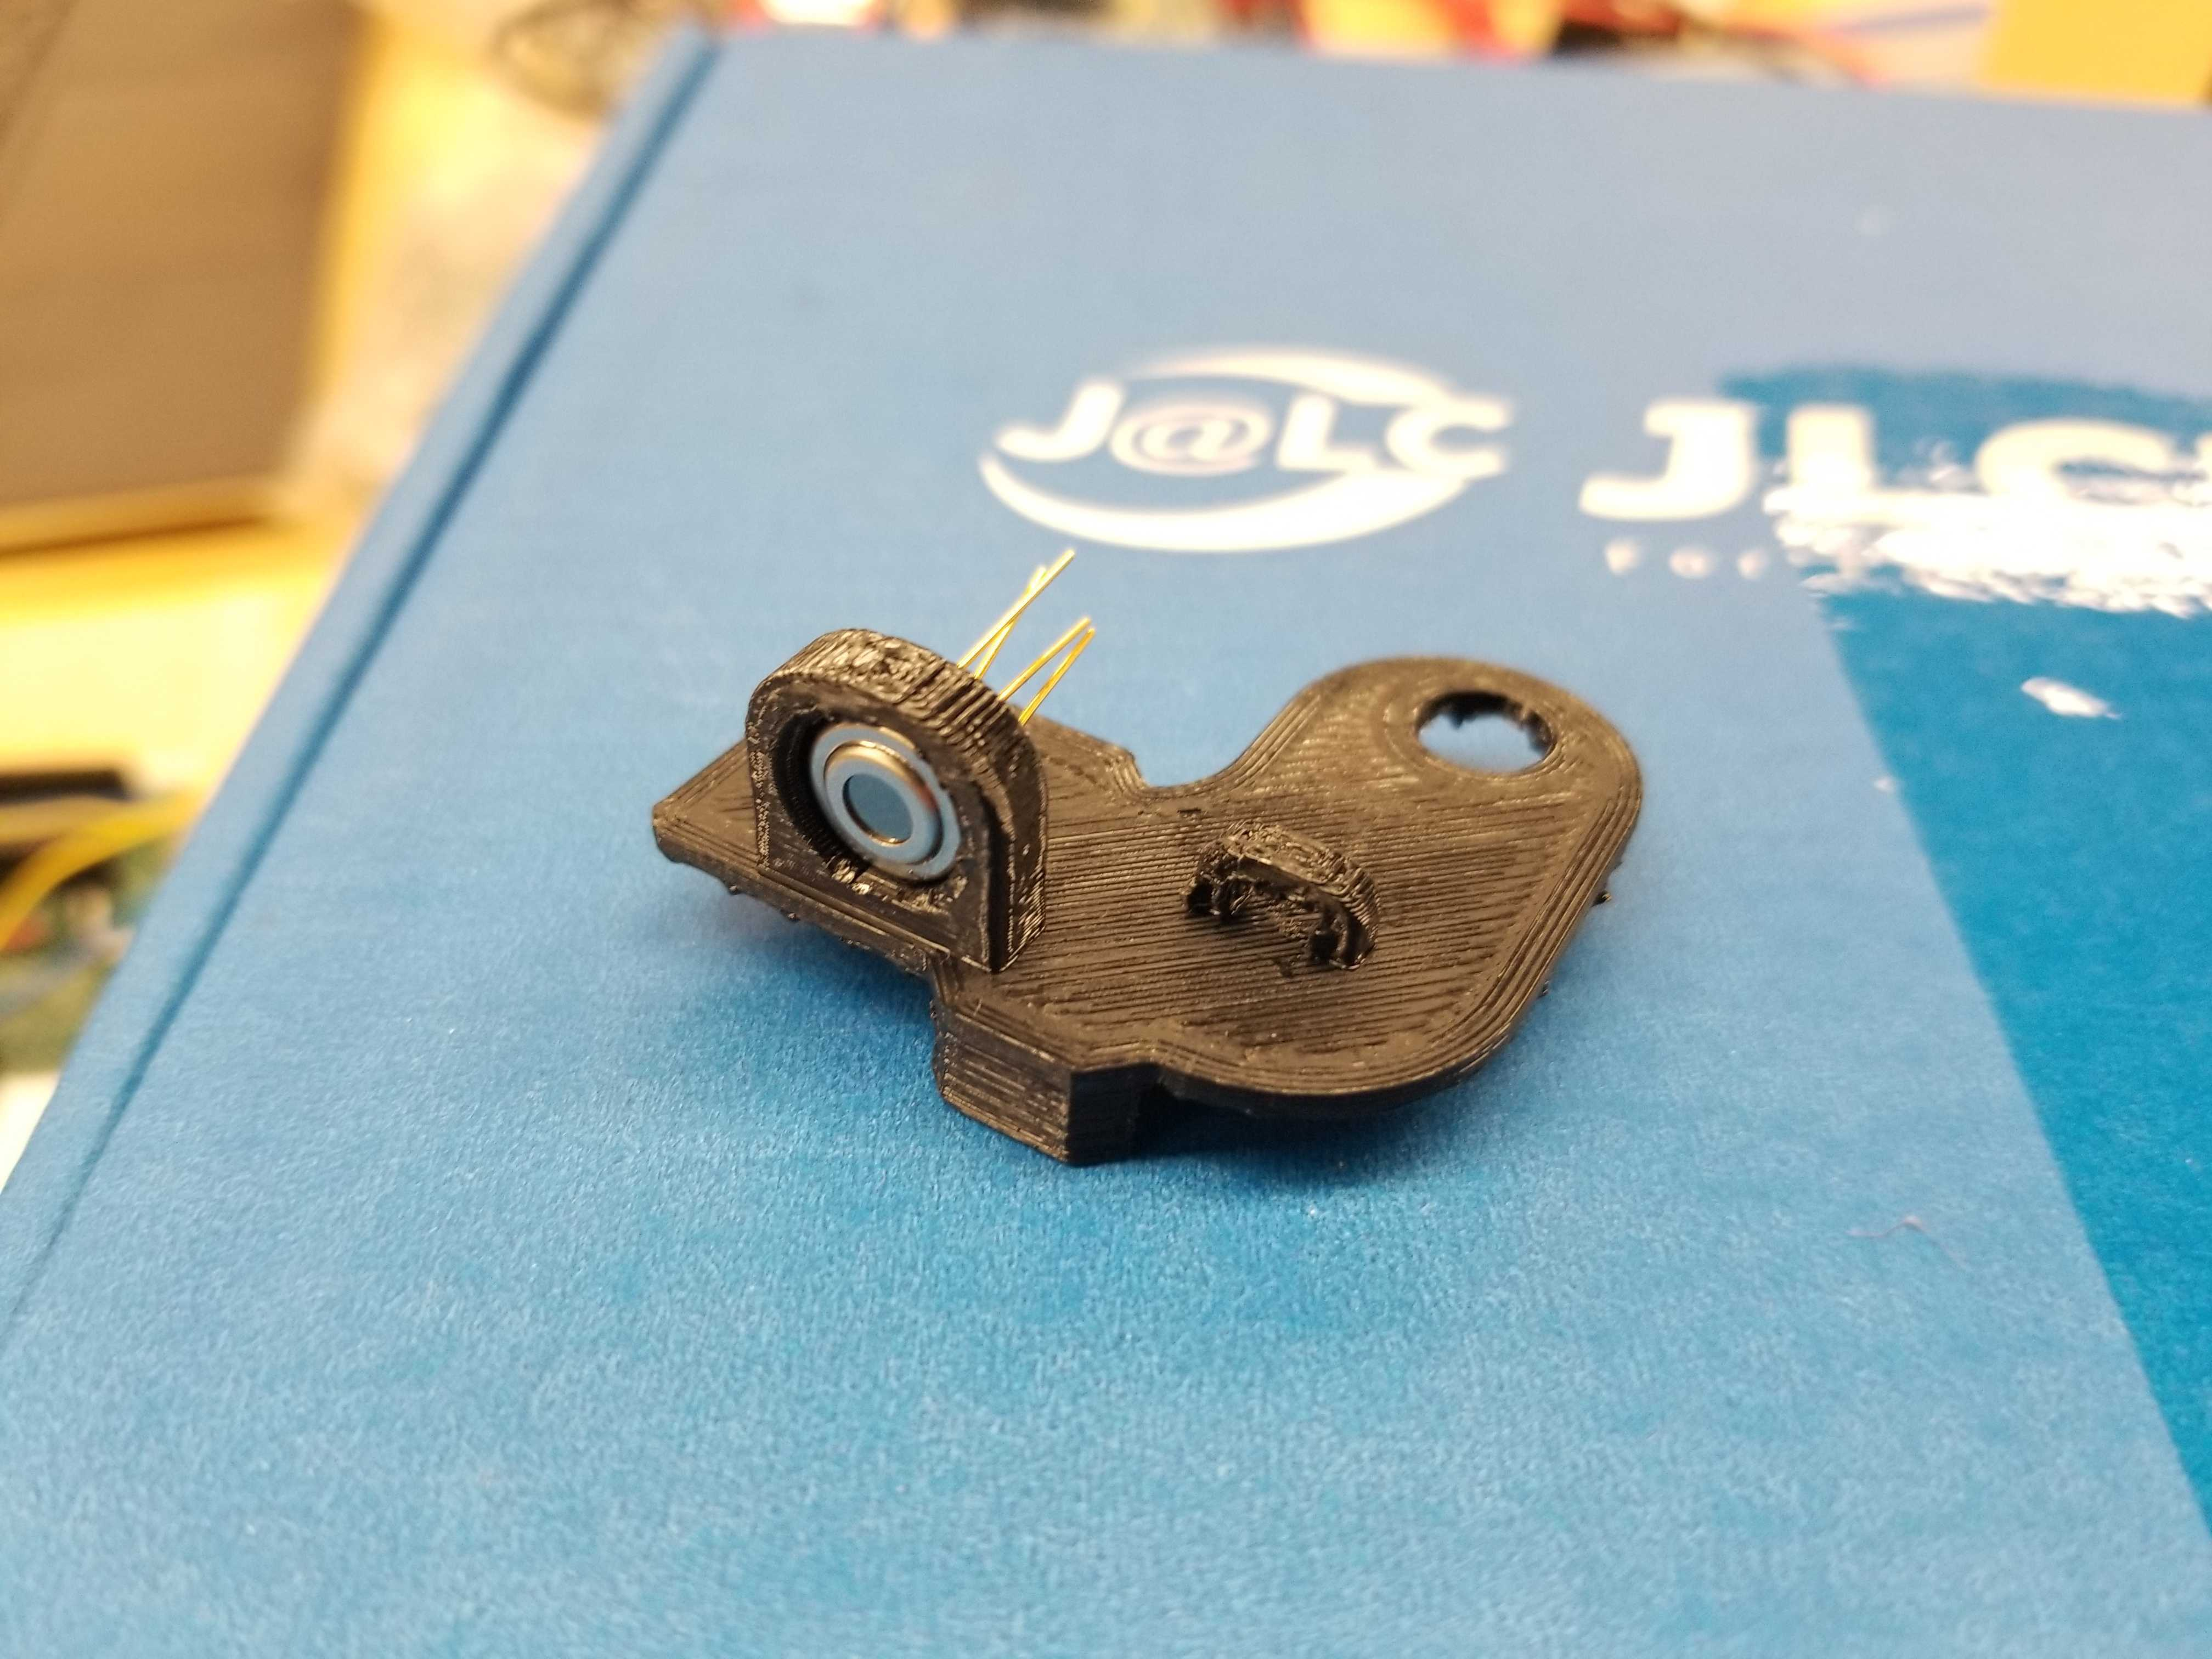
\includegraphics[width=3in]{images/brakes.jpg}
    \caption{Front Brake Temperature Sensor}
    \label{fig:fbts}
\end{figure}
\begin{figure}[H]
    \centering
    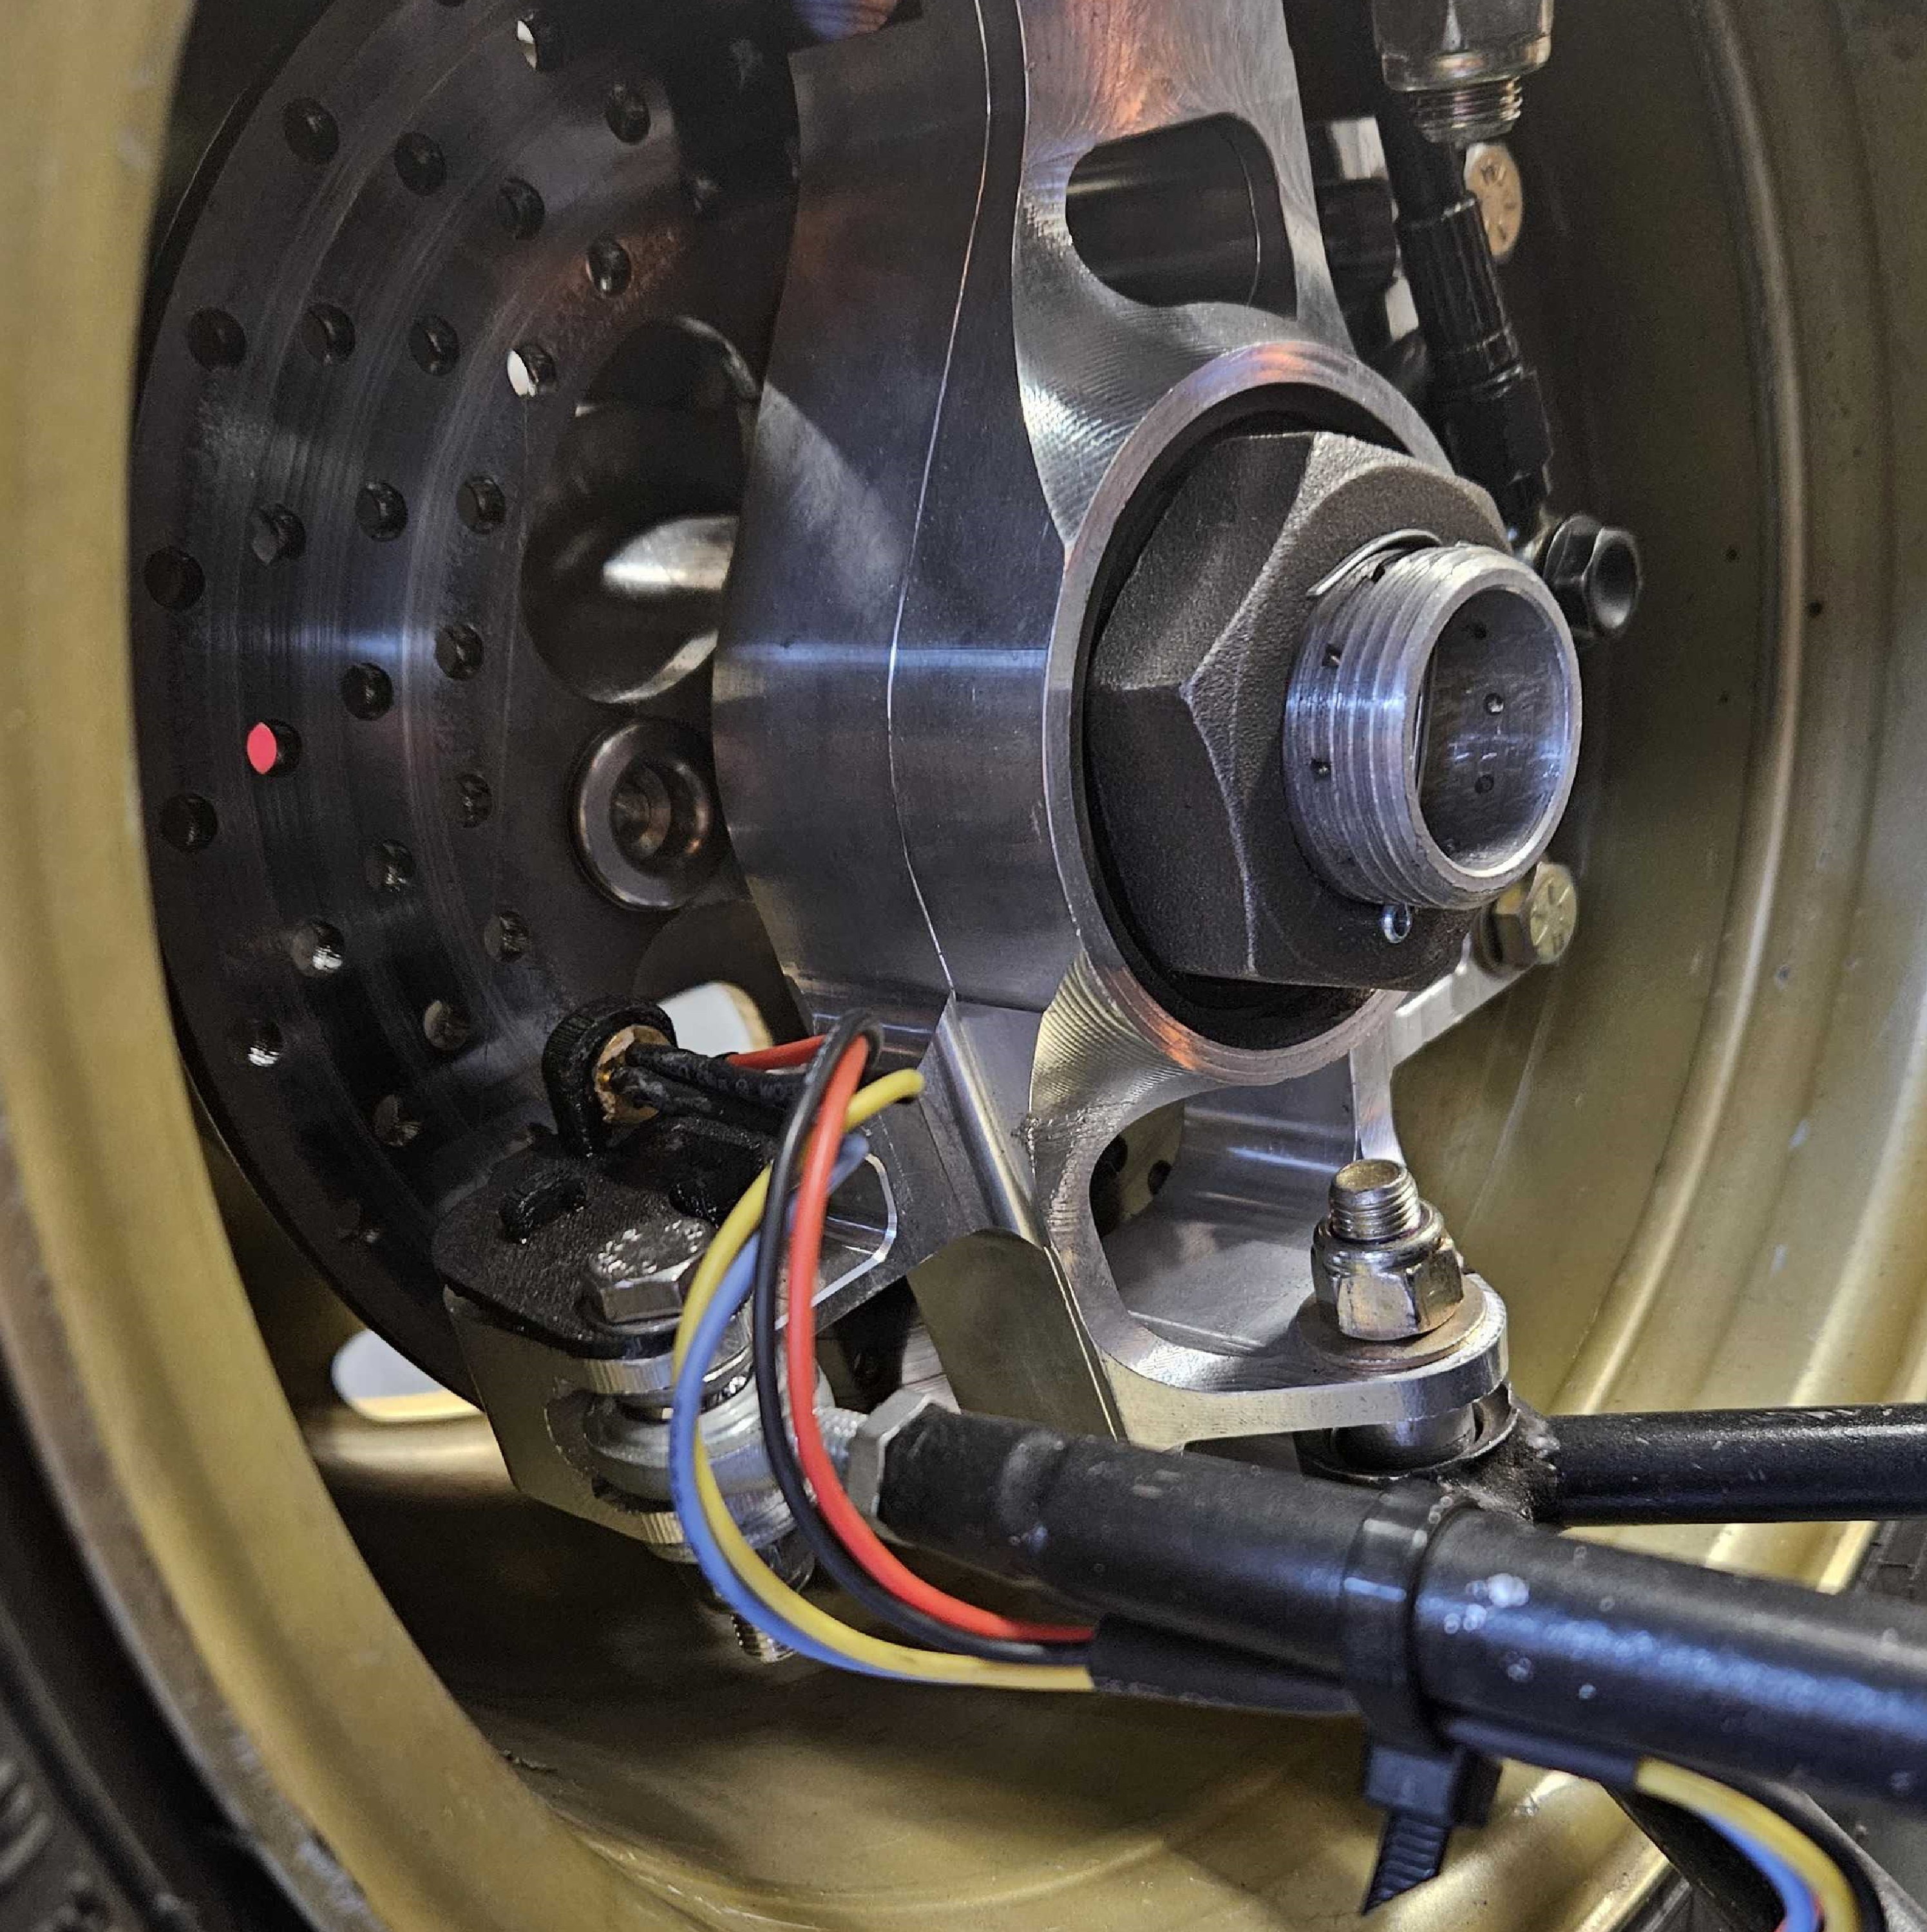
\includegraphics[width=5in]{images/brak.jpg}
    \caption{Installed Brake Temperature Sensor}
    \label{fig:ifbts}
\end{figure}
The MLX90614 library provided by Sparkfun was used to interact with the sensor.
\section{Strain Gauge Amplifier Design}
Although it is possible to hook up the output of a Wheatstone bridge directly to a microcontroller, the voltage difference produced by a bridge is often very minute.
As such, an amplifier board is required to get more precise data out of the bridge.
\vspace{1em}

The design for the strain gauge amplifier board was largely based off of the reference schematic from the HX711's datasheet.
The primary differences are that a Wheatstone bridge completion in a half bridge configuration is present, as well as a jumper to select the data rate.
To ensure the accuracy of the strain gauge, 1\% tolerance resistors were chosen to complete the bridge despite the fact that these are much more expensive.
Since this was the team's first time using the HX711 (or any strain gauge amplifier for that matter), a jumper to select the data rate was included to make the amplifier as flexible as possible.
\begin{figure}[H]
    \centering
    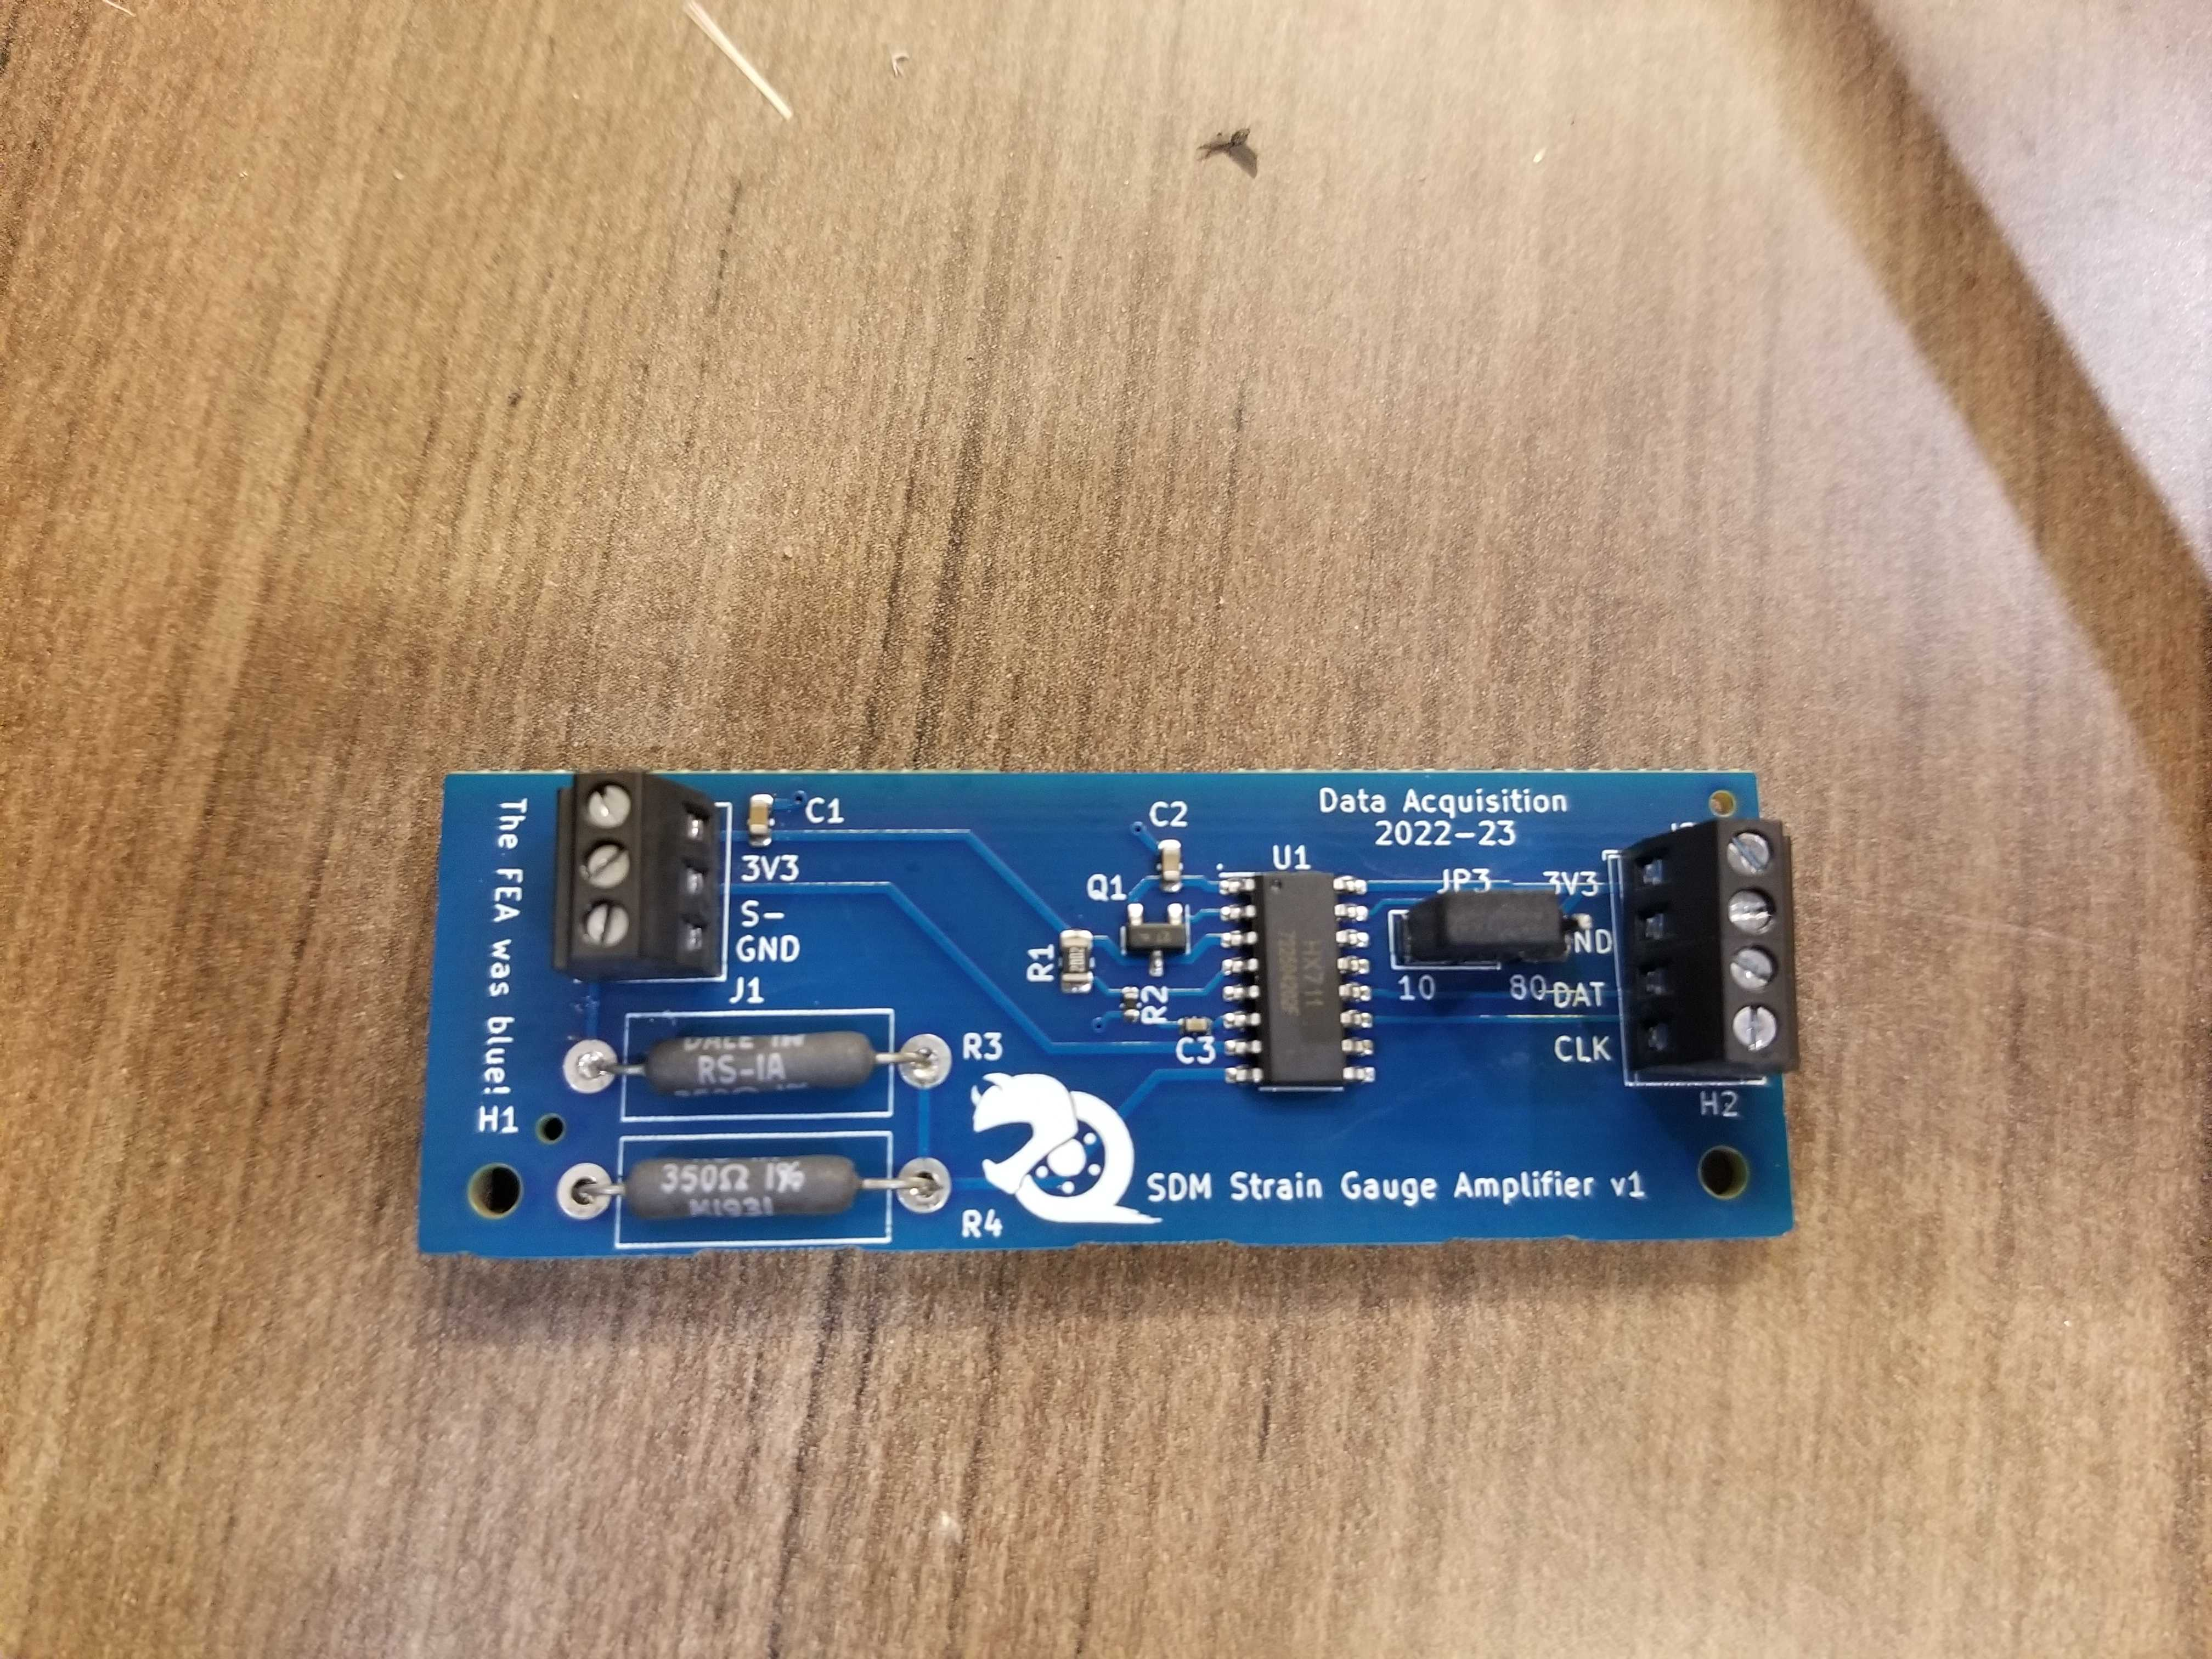
\includegraphics[width=4in]{images/sgamplifier-assembled.jpg}
    \caption{Strain Gauge Amplifier Board}
    \label{fig:sgb}
\end{figure}
A simple enclosure for the board was designed and printed using PETG.
\begin{figure}[H]
    \centering
    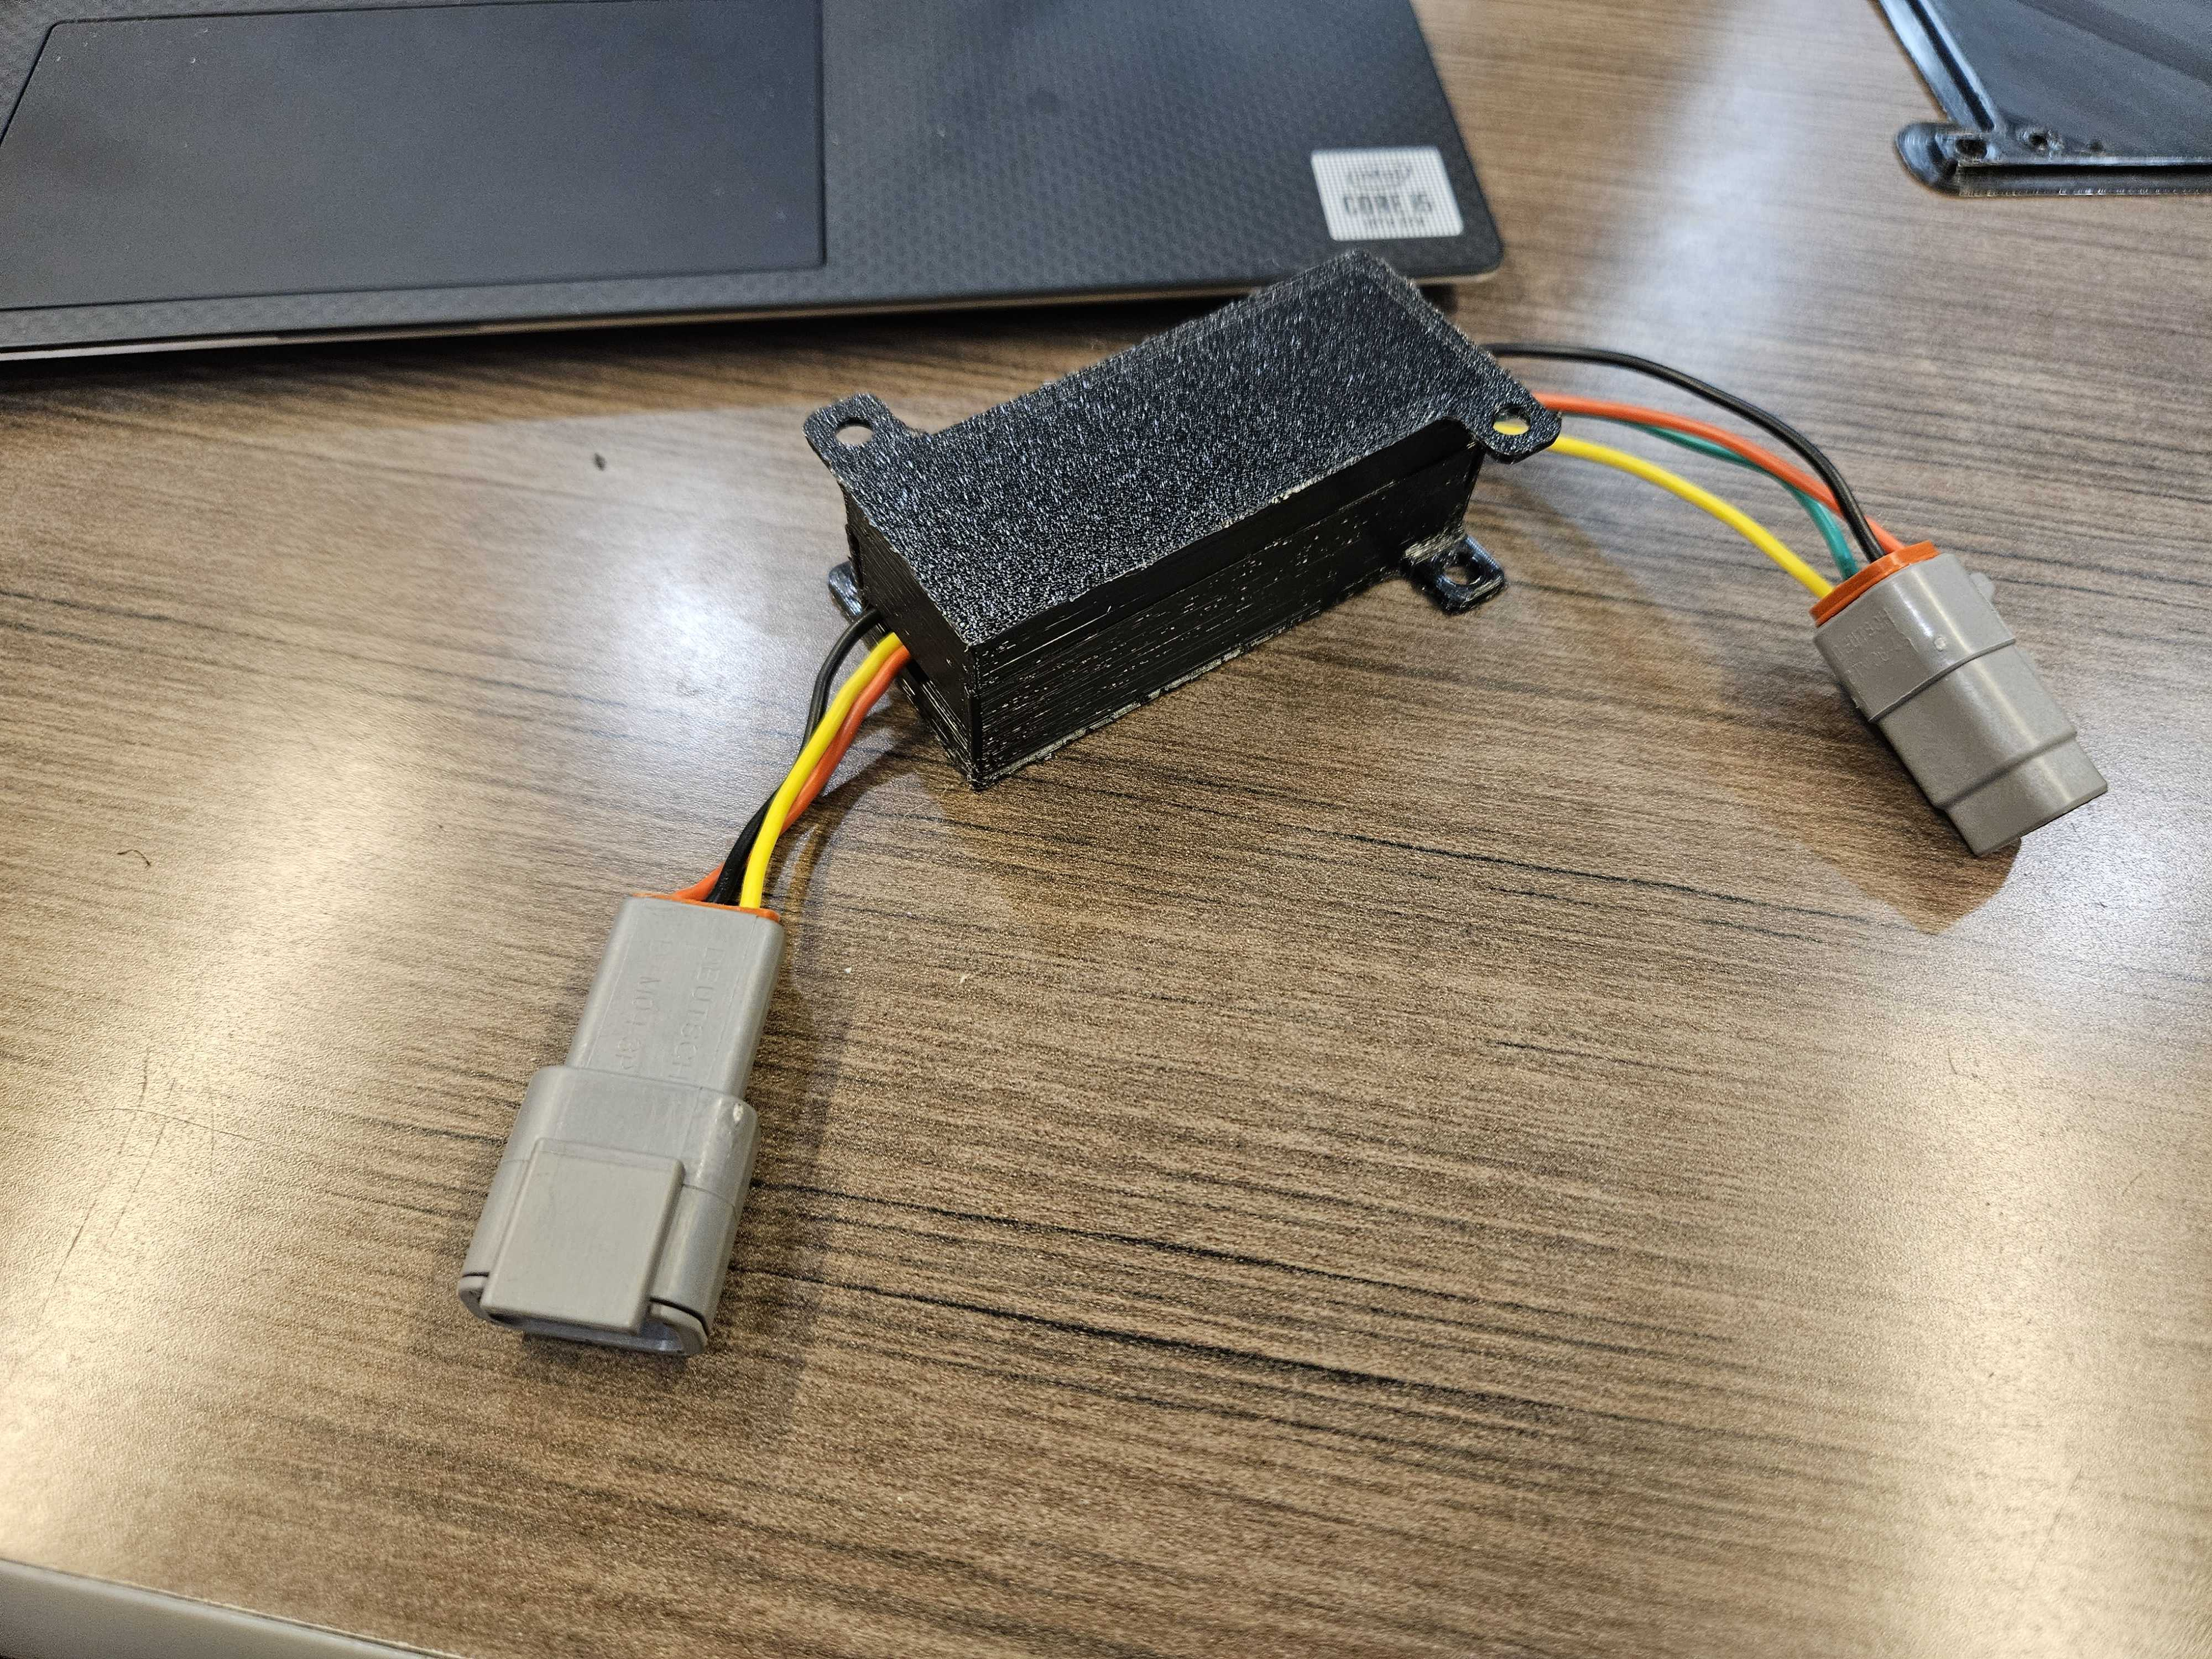
\includegraphics[width=3in]{images/sg-box.jpg}
    \caption{Strain Gauge Amplifier Box}
    \label{fig:sgxb}
\end{figure}

\section{Analysis Software Design}
A collection of software scripts have been developed in order to streamline the data processing pipeline as much as possible.
\begin{figure}[H]
    \centering
    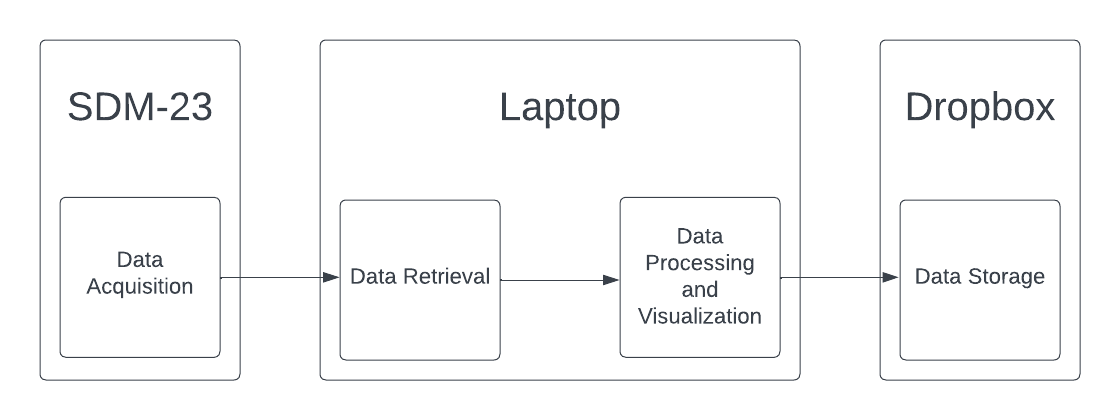
\includegraphics[width=5in]{images/SDM23DataPipeline.png}
    \caption{Data Processing Pipeline}
    \label{fig:dpp}
\end{figure}

\subsection{Data Retrieval}
The primary way of data retrieval is by turning the system off, taking the microSD card and copying the files over to a laptop, then replacing the microSD card in the system.
Although this is a reliable way of retrieving data, given that the main box needs to be disassembled in order to do so does not mean that it is an easy way.
As such, a set of scripts have been developed to retrieve data from the system by plugging the Main box into a laptop via USB:
\begin{itemize}
    \item Discovering Serial Ports
    \item Listing Files
    \item Download All Files
    \item Download Specific File
\end{itemize}
All scripts (with the exception of the discover ports script) follow the general format:
\begin{figure}[H]
    \centering
    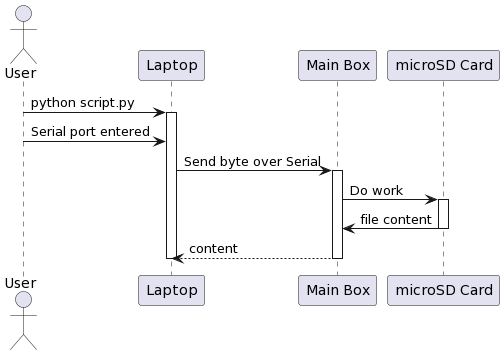
\includegraphics[width=5in]{images/dataretrieval-seq.png}
    \caption{Data Retrieval Script Sequence Diagram}
    \label{fig:drssd}
\end{figure}
The discover ports script is used to determine which serial port to input for the latter three scripts.
The list files script is used to view the files currently on the SD card and can be used in conjunction with the download specific file script, which downloads a specific file onto the laptop.
The last script downloads all files on the SD card onto the laptop.
\begin{figure}[H]
    \centering
    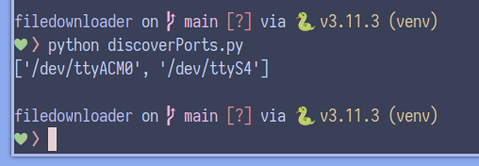
\includegraphics[width=4in]{images/discover.png}
    \caption{Discover Serial ports script output}
    \label{fig:dspsoi}
\end{figure}
\begin{figure}[H]
    \centering
    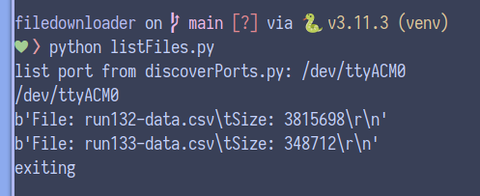
\includegraphics[width=4in]{images/list.png}
    \caption{List files script output}
    \label{fig:list}
\end{figure}
\begin{figure}[H]
    \centering
    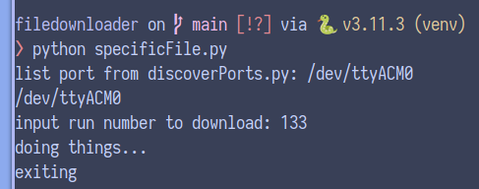
\includegraphics[width=4in]{images/specific.png}
    \caption{Download specific file script output}
    \label{fig:specific}
\end{figure}
\begin{figure}[H]
    \centering
    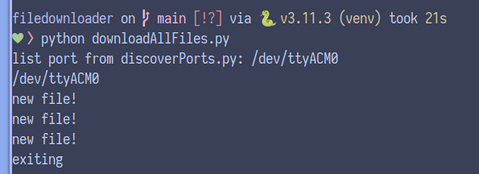
\includegraphics[width=4in]{images/all.png}
    \caption{Download all files script output}
    \label{fig:all}
\end{figure}
\subsection{Data Processing and Visualization}
Once data has been retrieved from the car, it is moved into a standardized directory structure seen in Figure \ref{fig:dir_struct}:
\begin{figure}[H]
    
    \dirtree{%
    .1 YYMMDD Track Day.
    .2 raw\DTcomment{Folder containing raw data retrieved from DAQ system}.
    .3 morning-session.
    .4 run9-data.csv.
    .4 run10-data.csv.
    .3 arb-test.
    .4 session1.
    .5 run11-data.csv.
    .5 run12-data.csv.
    .4 session2.
    .5 run13-data.csv.
    .5 run14-data.csv.
    .2 interim\DTcomment{Contains processed data with correct units}.
    .3 morning-session.
    .4 run9-data.csv.
    .4 run10-data.csv.
    .3 arb-test.
    .4 session1.
    .5 run11-data.csv.
    .5 run12-data.csv.
    .4 session2.
    .5 run13-data.csv.
    .5 run14-data.csv.
    .2 reports\DTcomment{Contains reports and plots for other subteams}.
    .3 morning-session.
    .4 run9-ggplot.png.
    .3 morning-summary.txt.
    .3 arb-test-session1-summary.txt.
    .3 arb-test-session2-summary.txt.
    .2 generate-ggplot.py.
    .2 generate-summary.py\DTcomment{Creates summary files for raw data}.
    .2 process.py\DTcomment{Processes raw data files to create interim files}.
    .2 requirements.txt\DTcomment{contains Python packages required to run scripts}.
    }
    \caption{Example Directory Structure for Data Processing}
    \label{fig:dir_struct}
\end{figure}
\subsubsection{Summary Generation}
Oftentimes during a testing session, run files are created that are not important to look at, such as when the car is idling or when the car is power cycled.
In order to parse through the run files more efficiently and throw out useless files, a script was created to generate summaries for each run file.
These summaries would include maximum values, ranges and other metrics that can be used to determine if a run file is worth looking closer into.
These metrics include:


\begin{itemize}
    \item maximum absolute lateral acceleration value
    \item minimum and maximum acceleration value
    \item brake pressure range
    \item maximum brake rotor temperature
    \item damper travel range
    \item maximum GPS ground speed value
    \item GPS fix acquired time
    \item Run file duration
\end{itemize}
\begin{figure}[H]
    \centering
    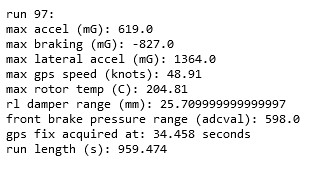
\includegraphics[width=4in]{images/summary.jpg}
    \caption{Example Run File Summary}
    \label{fig:sum}
\end{figure}
At the end of each summary, various lists of run numbers are created to give an overview of what run files fulfill a given metric.
\begin{figure}[H]
    \centering
    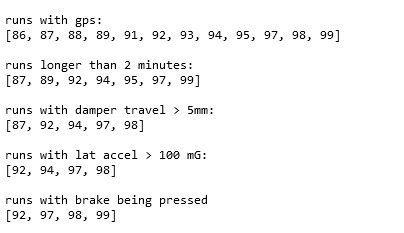
\includegraphics[width=4in]{images/sessionsumarry.jpg}
    \caption{Example Session Summary}
    \label{fig:sessionsumum}
\end{figure}
The summary files also give insight into any issues the DAQ system may have had while collecting data.
For instance if a box had power issues or a sensor was malfunctioning, the summary file would generally be able to catch that.
\subsubsection{Interim File Generation}
After summary files have been created, a script is used to generate interim run files.
These interim files have corrected units (e.g., for a steering angle sensor, the channel would have degrees instead of the raw ADC value) and drop any unused columns.
As such these are better suited to use for creating plots and diagrams as opposed to the raw files produced by the DAQ system.
\vspace{1em}

The \texttt{pandas} library is used to process and generate interim files.
\subsubsection{Plot and Diagram Generation}
A function was created for each kind of plot or diagram that was to be made, which would take a path, run number, and a force boolean as input.
If the force boolean evaluated to false, then simple criteria would be used to determine if a plot for the given run number and path would be generated, which was useful for automatically generating plots.
For example if the plot was brake rotor temperature vs time, then a check for the rotor temperature range would determine if a plot would be generated or not.
\vspace{1em}

\texttt{matplotlib} and \texttt{pandas} are used for plot and diagram generation.

\subsubsection{Lap Generation}
It is important to create a distinction between laps and laptimes during tests/races. Data visualization is a process which encapsulates this need and enables the ability to better our results through data. Using GPS data consisting of latitude/longitude alongside timestamps, we can acquire this data.
The lap generation program uses python notebooks utilizing pandas and matplotlib and encapsulates the data from csv in a dataframe. Our determination of a new lap utilizes a radius from the beginning point where this acts as a threshold to determine whenever the car passes this point. To determine whether the current point is within the threshold, the distance between points needs to be calculated. The calculation determines the distance between the first node detected and the current node within the dataframe. The equation is as follows:
\begin{gather}
    D_{a,b} = \sqrt{(\Delta latitude)^2 + (\Delta longitude)^2} 
\end{gather}

Once a distance between two points is acquired, we compare this to our selected radius threshold to determine whether our lap counter should be incremented. Iterating through our dataframe with the process described above will yield the ability to count the number of laps quantitatively and as well enable us to visualize the laps on a map. This visualization can be seen in a multitude of ways. To visualize how our laps are counted, one can plot a distance vs time graph where distance is the displacement of the car from a arbitrarily chosen location. A sample graph is provided: 

\begin{figure}[H]
    \centering
    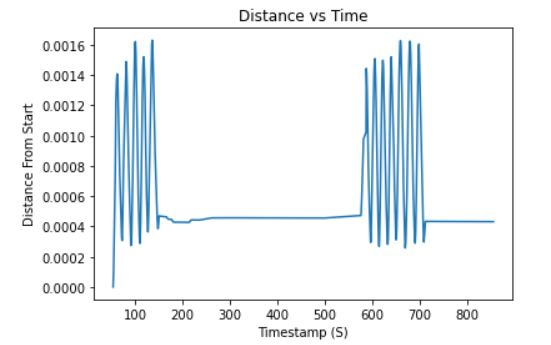
\includegraphics[width=5in]{images/distancevtime.png}
    \caption{Distance vs Time Graph}
    \label{fig:dtg}
\end{figure}

\vspace{1em}

Additionally, there is a possible roadmap for where this track map can go. Firstly, we can overlay the laps on to a map provided by openstreetmap and see where our data was gathered geographically. While not impressive currently, this provides the framework for the team to expand upon this idea to sort and parse this data to make it more viable for the team. Examples of this should include showing singular laps at a time, color-coding based on lateral acceleration, and viewing racing lines. A picture of this is provided:

\begin{figure}[H]
    \centering
    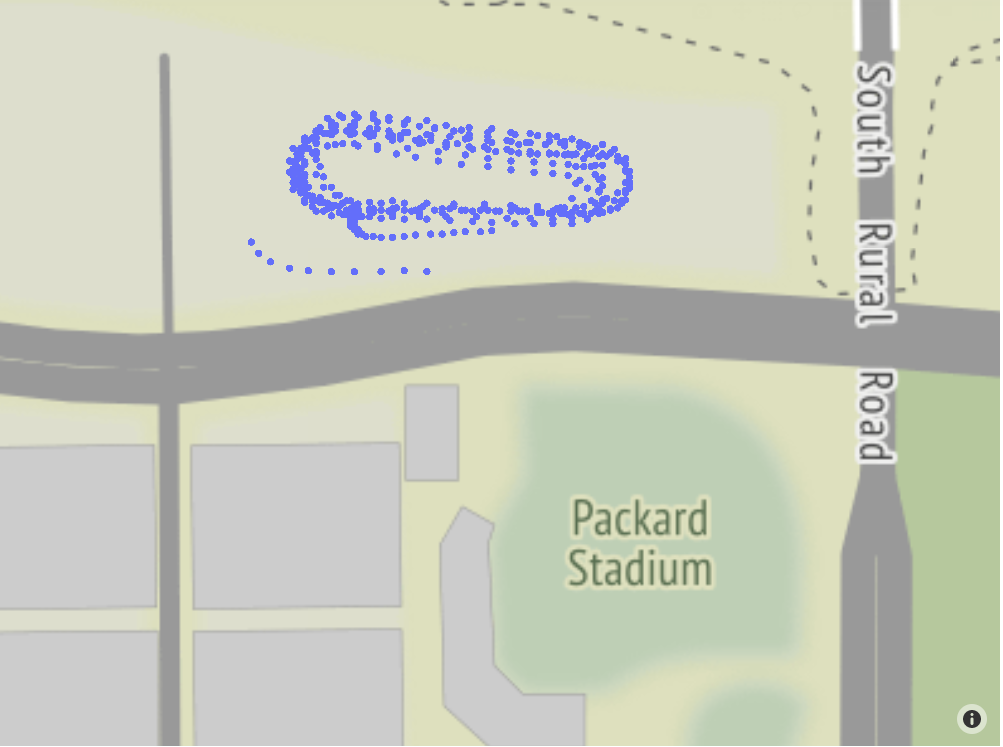
\includegraphics[width=5in]{images/map.png}
    \caption{OpenStreetView Map}
    \label{fig:osvm}
\end{figure}

\subsection{Data Storage}
All raw and interim files, as well as any generated reports and notes, are stored on the team's Dropbox and can be viewed and downloaded by anyone on the team with access to it.
For SDM-23 Track Day data, a directory spreadsheet was created to help the team find data they are looking for.
This directory includes:
\begin{itemize}
    \item Date of track day
    \item A Data Quality Rating
    \item Sensor availability
    \item Notes
    \item Link to data folder in Dropbox
\end{itemize}
The Data Quality Rating is a rating from 1 (unusable) to 10 (good) based on how reliable the DAQ system was for the given track day that was qualitatively determined by the DAQ subteam.
The sensor availability chart gives a simple rating for each sensor.
If the cell is green, then the data produced by the sensor was consistent and likely usable.
If the cell is yellow, then the data produced was of mixed quality, or is partially missing.
If the cell is red then no data was collected from that sensor for the given track day.

These two metrics and the testing notes give an overview for team members to easily determine and find where data for a given track day is.
\begin{figure}[H]
    \centering
    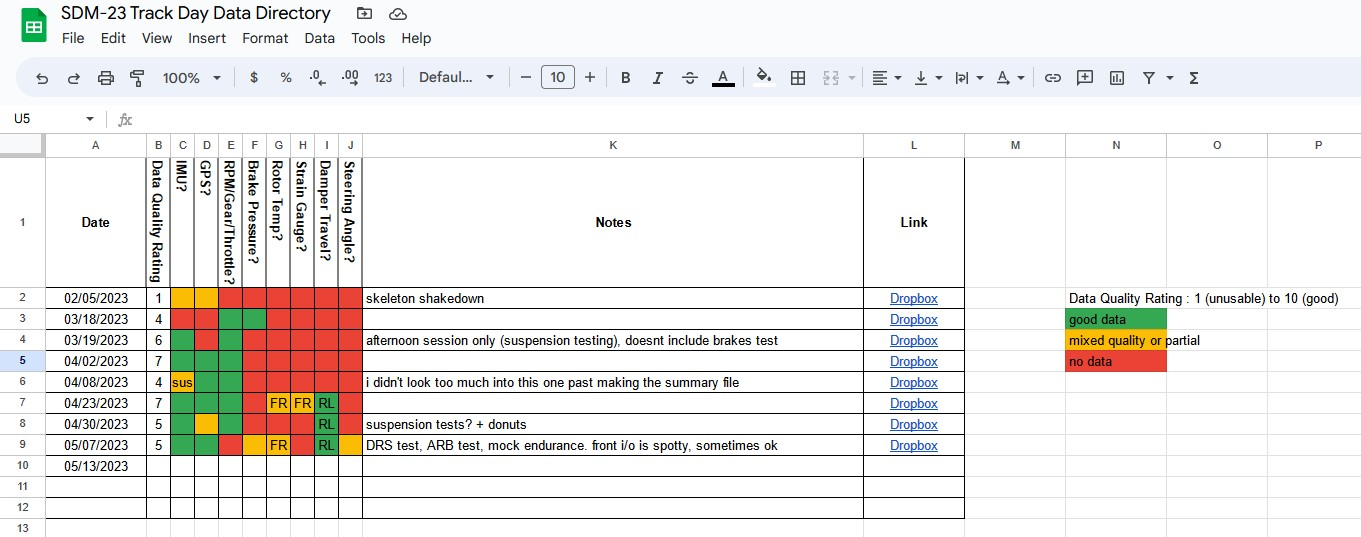
\includegraphics[width=7in]{images/tddr.jpg}
    \caption{SDM-23 Track Day Data Directory}
    \label{fig:tddr}
\end{figure}
